\documentclass{warpdoc}
\newlength\lengthfigure                  % declare a figure width unit
\setlength\lengthfigure{0.158\textwidth} % make the figure width unit scale with the textwidth
\usepackage{psfrag}         % use it to substitute a string in a eps figure
\usepackage{subfigure}
\usepackage{rotating}
\usepackage{pstricks}
\usepackage[innercaption]{sidecap} % the cute space-saving side captions
\usepackage{scalefnt}
\usepackage{amsbsy}
\usepackage{bm}
\usepackage{amsmath}
\usepackage{multirow}
\usepackage{longtable}
\usepackage[hidelinks]{hyperref} %added by Prasanna

%%%%%%%%%%%%%=--NEW COMMANDS BEGINS--=%%%%%%%%%%%%%%%%%%%%%%%%%%%%%%%%%%
\newcommand{\alb}{\vspace{0.1cm}\\} % array line break
\newcommand{\rhos}{\rho}
\newcommand{\cv}{{c_v}}
\newcommand{\cp}{{c_p}}
\newcommand{\Sct}{{{\rm Sc}_{\rm T}}}
\newcommand{\Prt}{{{\rm Pr}_{\rm T}}}
\newcommand{\nd}{{{n}_{\rm d}}}
\newcommand{\ns}{{{n}_{\rm s}}}
\newcommand{\nn}{{{n}_{\rm n}}}
\newcommand{\ndm}{{\bar{n}_{\rm d}}}
\newcommand{\nsm}{{\bar{n}_{\rm s}}}
\newcommand{\turb}{_{\rm T}}
\newcommand{\mut}{{\mu\turb}}
\newcommand{\mfa}{\scriptscriptstyle}
\newcommand{\mfb}{\scriptstyle}
\newcommand{\mfc}{\textstyle}
\newcommand{\mfd}{\displaystyle}
\newcommand{\hlinex}{\vspace{-0.34cm}~~\\ \hline \vspace{-0.31cm}~~\\}
\newcommand{\hlinextop}{\vspace{-0.46cm}~~\\ \hline \hline \vspace{-0.32cm}~~\\}
\newcommand{\hlinexbot}{\vspace{-0.37cm}~~\\ \hline \hline \vspace{-0.50cm}~~\\}
\newcommand{\tablespacing}{\vspace{-0.4cm}}
\newcommand{\fontxfig}{\footnotesize\scalefont{0.918}}
\newcommand{\fontgnu}{\footnotesize\scalefont{0.896}}
\renewcommand{\fontsizetable}{\footnotesize\scalefont{1.0}}
\renewcommand{\fontsizefigure}{\footnotesize}
%\renewcommand{\vec}[1]{\pmb{#1}}
%\renewcommand{\vec}[1]{\boldsymbol{#1}}
\renewcommand{\vec}[1]{\bm{#1}}
\setcounter{tocdepth}{3}
\let\citen\cite
\newcommand\frameeqn[1]{\fbox{$\displaystyle #1$}}

%%%%%%%%%%%%%=--NEW COMMANDS BEGINS--=%%%%%%%%%%%%%%%%%%%%%%%%%%%%%%%%%%

\setcounter{tocdepth}{3}

%%%%%%%%%%%%%=--NEW COMMANDS ENDS--=%%%%%%%%%%%%%%%%%%%%%%%%%%%%%%%%%%%%



\author{
  Bernard Parent and Prasanna Thoguluva Rajendran
}

\email{
  bparent@arizona.edu
}

\department{
  Aerospace and Mechanical Engineering	
}

\institution{
  University of Arizona
}

\title{
  Transport Coefficients
}

\date{
  1998--2022
}

%\setlength\nomenclaturelabelwidth{0.13\hsize}  % optional, default is 0.03\hsize
%\setlength\nomenclaturecolumnsep{0.09\hsize}  % optional, default is 0.06\hsize

\nomenclature{

  \begin{nomenclaturelist}{Roman symbols}
   \item[$a$] speed of sound
  \end{nomenclaturelist}
}


\abstract{
abstract
}

\begin{document}
  \pagestyle{headings}
  \pagenumbering{arabic}
  \setcounter{page}{1}
%%  \maketitle
  \makewarpdoctitle
%  \makeabstract
  \tableofcontents
%  \makenomenclature
%%  \listoftables
%%  \listoffigures


\section{Effect of Electric Field on Mobilities}


%
\begin{table*}[t]
  \center
  \begin{threeparttable}
    \tablecaption{Effect of electric field on electron and ion mobilities.\tnote{a}}
    \label{tab:mobilities:Ecorrection}
    \fontsizetable
    \begin{tabular*}{\textwidth}{l@{\extracolsep{\fill}}ll}
    \toprule
    Species & Corrected Mobility, $\rm m^2\cdot V^{-1}\cdot s^{-1}$  & Reference\\
    \midrule
    N$_2^+$         & $\min\left( \mu_{\rm N_2^+},~~N^{-1}\cdot 2.03 \cdot 10^{12}\cdot \left(E^\star\right)^{-0.5} \right)$  & \cite{misc:1968:sinnott}\alb
    O$_2^+$         &  $\min \left( \mu_{\rm O_2^+},~~N^{-1}\cdot 3.61 \cdot 10^{12}\cdot\left(E^\star\right)^{-0.5}\right)$  & \cite{misc:1968:sinnott}\alb
    O$_2^-$         & $\min \left( \mu_{\rm O_2^-},~~N^{-1}\cdot 3.56 \cdot 10^{19} \cdot \left(E^\star\right)^{-0.1}\right)$  & \cite{misc:1983:gosho}\alb
    other~ions         & $\min\left( \mu_{\rm i},~~N^{-1}\cdot 0.55 \cdot \left(m_{\rm i} E^\star\right)^{-0.5}\right)$  & --\alb
    e$^-$         & \begin{tabular}{@{}l}$(1-\xi)\cdot \mu_{\rm e} + \xi \cdot N^{-1} \cdot \left(4\cdot 10^{19}\cdot(-30 -\ln E^\star)^4+1.3\cdot 10^{40}\cdot E^\star\right) $\\~~~~with~$\xi=\max\left(0,~\min(1,~19+\log_{10}E^\star)\right)$\end{tabular}  & \cite{ps:2005:tarasenko}\tnote{b}\\
    \bottomrule
    \end{tabular*}
    \begin{tablenotes}
      \item[a] Notation and units:  $m_{\rm i}$ is the mass of one ion particule in kg; $N$ is the total number density of the plasma in 1/m$^3$; $E^\star$ is the reduced effective electric field  ($E^\star \equiv |\vec{E}|/N$) in units of V$\cdot$m$^2$; $\mu_k$ is the uncorrected mobility of species $k$ in $\rm m^2\cdot V^{-1}\cdot s^{-1}$.
      \item[b] The electron mobility weight factor $\xi$ is such that the corrected mobility is a blend of the uncorrected mobility (function of electron temperature only) and the high-electric-field mobility (function of reduced electric field only) in the range $10^{-19}<E^\star<10^{-18}~ {\rm Vm^2}$. In the range $E^\star>10^{-19}~ {\rm Vm^2}$ the corrected mobility is simply set equal to the high-electric-field mobility. Note that the corrected mobility data outlined in \cite{ps:2005:tarasenko} is valid for $10^{-19}<E^\star<5\cdot 10^{-17}$~Vm$^2$.
    \end{tablenotes}
   \end{threeparttable}
\end{table*}
%

Electron and ion mobilities are function not only of ion or electron temperature but also of the reduced electric field. This can be explained as follows. Consider first the electron mobility. In high $E$-field discharges or in electron beams, the electron temperature (i.e.\ defined as being proportional to the average kinetic energy of the electrons with respect to the electron bulk motion) ceases to have a meaningful impact on chemical reactions between electrons and heavier particules. This is because the main source of velocity difference between electrons and heavy particules is the drift of the electrons with respect to the gas. Because the electron drift velocity is function of the reduced electric field, the electron mobility also becomes function mostly of the electric field (and not electron temperature) when the reduced electric field is high. Similar arguments can be made for the ions. As the reduced electric field becomes large, the ion mobility is less function of ion temperature but more function of the ion drift because the main source of velocity difference between the ions and the neutrals is the drift of the ions, not the ions thermal velocity. Thus, in discharges where the electric field is high, the ion mobility should be function of the reduced electric field.

The effect of the electric field on the electron and ion mobilities is taken from various sources and tabulated in Table \ref{tab:mobilities:Ecorrection}. 



\section{Mass Diffusion Coefficients from Binary Diffusion Coefficients}

Transport models by Dixon-Lewis or by Gupta-Yos will give expressions for the binary diffusion coefficients $D_{ij}$. However, those need to be converted into a mass diffusion coefficient $\nu_k$ in order to be implemented in a CFD code. There are several ways to do this, with varying amount of computing and accuracy.

\subsection{Oran-Boris Mass Diffusion Model}

One of the simplest mass diffusion coefficient model is the one outlined in Oran-Boris \cite{pces:1981:oran}.
The molecular diffusion coefficient of species $k$, $\nu_k$,
is found from the binary diffusion coefficients as follows \cite[Eq.\ (6.15)]{pces:1981:oran}:
%
\begin{equation}
\mfd\nu_k= \frac{\rhos \left( 1 - {\chi}_k \right)}
            {\mfd\sum_{\mfa l=1..\ns}^{l \neq k} \frac{{\chi}_l}{{\cal D}_{k,l}} +10^{-20}   }
\label{eqn:moldiff-nu}
\end{equation}
%
In the latter, the molar fraction can be found from the mass fractions as follows:
%
\begin{equation}
{\chi}_k= \mfd\frac{w_k / {\cal M}_k}
              {\mfd\sum_{\mfa l=1}^{\ns} \left( w_l / {\cal M}_l \right)}
\end{equation}
%
where $w_k$ is the mass fraction. 

\subsection{Ramshaw-Shang SCEBD Mass Diffusion Model}

Another model is the SCEBD (Self-Consistent Effective Binary Diffusion) model by Ramshaw and Shang \cite{jnet:1996:ramshaw}.








\section{Gupta-Yos Transport Coefficients}

In the paper by Gupta, Yos, et al. \cite{nasa:1990:gupta}, various methods are outlined to determine the viscosity, thermal conductivity, and diffusion coefficients of a gas mixture. 

\subsection{Mixture Viscosity}

The viscosity of the mixture is found using an approximation to the first Chapman-Enskog model:
%
\begin{equation}
    \eta=\frac{\mfd\sum_{i=1}^{n_s} \frac{\chi_i}{A_i+a_{\rm av}}}{\mfd 1- a_{\rm av}\sum_{i=1}^{n_s}\frac{\chi_i}{A_i + a_{\rm av}}}
\end{equation}
%
with $\eta$ the viscosity in gm/cm-sec. In the latter, $\chi_i$ is the molar fraction of the $i$th species, $n_s$ the number of species (including ions and electrons), and  $a_{\rm av}$ is defined as:
%
\begin{equation}
  a_{\rm av}=\frac{\mfd\sum_{i=1}^{n_s} \sum_{j=1}^{n_s} \chi_i \chi_j \left(\frac{1}{A_i}- \frac{1}{A_j} \right)^2 a_{ij}}{\mfd\sum_{i=1}^{n_s} \sum_{j=1}^{n_s} \chi_i \chi_j \left( \frac{1}{A_i} - \frac{1}{A_j}\right)^2}
\end{equation}
%
with:
%
\begin{equation}
    A_i= \sum_l^{n_s}  \chi_l \frac{N_{\rm A}}{{\cal M}_i} \Delta_{il}^{(2)}(T) 
\end{equation}
%
%
\begin{equation}
    a_{ij}=\frac{N_{\rm A}}{{\cal M}_i+{\cal M}_j}\left(2 \Delta_{ij}^{(1)}(T) - \Delta_{ij}^{(2)}(T) \right)
\end{equation}
%
with $N_{\rm A}$ the Avogadro number ($6.0221\times 10^{23}$ molecules per g-mole) and ${\cal M}_i$ the molecular weight of the $i$th species in gr/g-mole.

Also,
%
\begin{equation}
    \Delta_{ij}^{(1)}(T)=(\ln \Lambda)_{ij}\frac{8}{3} (1.5460 \times 10^{-20}) \pi \Omega_{ij}^{(1,1)}(T) \sqrt{\frac{2 {\cal M}_i {\cal M}_j}{\pi {\cal R} T ({\cal M}_i + {\cal M}_j)} }
\end{equation}
%
%
\begin{equation}
    \Delta_{ij}^{(2)}(T)=(\ln \Lambda)_{ij} \frac{16}{5} (1.5460 \times 10^{-20}) \pi \Omega_{ij}^{(2,2)}(T) \sqrt{\frac{2 {\cal M}_i {\cal M}_j}{\pi {\cal R} T ({\cal M}_i + {\cal M}_j)} }
\end{equation}
%
with $(\ln \Lambda)_{ij}$ the electron pressure correction which is set here to:
%
\begin{equation}
  (\ln \Lambda)_{ij}=\left\{ \begin{array}{ll}\mfd\frac{1}{2} \ln \left( \mfd 0.0209 \left( \frac{T_{\rm e}^4}{1000 P_{\rm e} }\right) + 1.52 \left( \frac{T_{\rm e}^4}{1000 P_{\rm e} }\right)^\frac{2}{3}
  \right)
  & \textrm{if species $i$ and $j$ and both charged}\\
  1 & {\rm otherwise}  
  \end{array}
  \right.
\end{equation}
%
with $P_{\rm e}$ the electron pressure in atm, $\cal R$ the universal gas constant in cal/(g-mol K), $T_{\rm e}$ the electron temperature in K, $T$ the heavy species temperature in K. Also, $\Omega_{ij}^{(1,1)}$ is the average collision cross-section (used for diffusion, viscosity, translational, internal, and reaction components of
thermal conductivity) for collisions between species $i$ and $j$ in square Angstroms. Similarly $\Omega_{ij}^{(2,2)}(T)$ is the average collision cross-section (used for viscosity and translational component of thermal conductivity) for collisions between species $i$ and $j$ in square Angstroms.  Expressions and data for $\Omega_{ij}^{(1,1)}(T)$ and $\Omega_{ij}^{(2,2)}(T)$ as a function of temperature can be found in \cite{nasa:1990:gupta}.

\subsection{Binary Diffusion Coefficients}

The binary diffusion coefficient corresponds to:
%
\begin{equation}
    {\cal D}_{ij}=\frac{1}{N \Delta_{ij}^{(1)}}
    \label{eqn:GY:Dij}
\end{equation}
%
with ${\cal D}_{ij}$ the binary diffusion coefficient in cm$^2$/s, $N$ the number density of the plasma in $1/{\rm cm}^3$ and $\Delta_{ij}^{(1)}$ has units of cm$\cdot$s.



\subsection{Species Thermal Conductivity}

The thermal conductivity of the electrons can be found from:
%
\begin{equation}
\frameeqn{
\kappa_{\rm e}=\frac{\frac{15}{4} \cdot 2.3901 \cdot 10^{-8} k_{\rm B} \chi_{\rm e}}{\sum_{j=1}^{n_{\rm s}-1}1.45 \chi_j \Delta_{ej}^{(2)}(T_e) +\chi_{\rm e} \Delta_{ee}^{(2)}(T_e)  }
}
\end{equation}
%
with $k_{\rm B}$ the Boltzman constant ($1.38066\cdot10^{-16}$~erg/K) and with $\kappa_{\rm e}$ in cal/cm-sec-K.
For a fully-excited  rotational state and partially excited vibrational and electronic states, the thermal conductivity of the heavy molecular species (neutrals or ions with more than 1 atom) is determined from:
%
\begin{equation}
\kappa_i = 
\frac{(2.3901\cdot10^{-8}) \frac{15}{4} k_{\rm B}  \cdot \chi_i}{3.54\cdot \chi_{\rm e} \Delta_{ie}^{(2)}(T_{\rm e})+ \sum_{j=1}^{n_s-1} \alpha_{ij} \chi_j \Delta_{ij}^{(2)}(T) }
+
\frac{(2.3901\cdot10^{-8}) k_{\rm B}  \cdot \chi_i}{ \chi_{\rm e} \Delta_{ie}^{(1)}(T_{\rm e})+\sum_{j=1}^{n_s-1} \chi_j \Delta_{ij}^{(1)}(T) }
\left(
\frac{(c_p)_{i}^{{\rm rot}}}{\cal R}+ \frac{(c_p)_{i}^{{\rm vib}}}{\cal R}
+ \frac{(c_p)_{i}^{{\rm elec}}}{\cal R}
\right)
\end{equation}
%
But note that the species specific heat at constant pressure corresponds to:
%
\begin{equation}
    (c_p)_i=(c_p)_i^{{\rm tr}}+(c_p)_i^{{\rm rot}}+(c_p)_i^{{\rm vib}}+(c_p)_{i}^{{\rm elec}}
\end{equation}
%
Also note that $(c_p)_{\rm tr}=\frac{5}{2}{\cal R}$. Then:
%
\begin{equation}
    (c_p)_i=\frac{5}{2}{\cal R}+(c_p)_i^{\rm rot}+(c_p)_i^{\rm vib}+(c_p)_i^{\rm elec}
\end{equation}
%
Divide by $\cal R$ and rearrange:
%
\begin{equation}
    \frac{(c_p)_i^{\rm rot}+(c_p)_i^{\rm vib}+(c_p)_i^{\rm elec}}{\cal R}=\frac{(c_p)_i}{\cal R}-\frac{5}{2}
\end{equation}
%
Substitute in the expression for $\kappa_i$ above:
%
\begin{equation}
\frameeqn{
\kappa_i = 
\frac{(2.3901\cdot10^{-8}) \frac{15}{4} k_{\rm B}  \cdot \chi_i}{3.54\cdot \chi_{\rm e} \Delta_{ie}^{(2)}(T_{\rm e})+ \sum_{j=1}^{n_s-1} \alpha_{ij} \chi_j \Delta_{ij}^{(2)}(T) }
+
\frac{(2.3901\cdot10^{-8}) k_{\rm B}  \cdot \chi_i}{ \chi_{\rm e} \Delta_{ie}^{(1)}(T_{\rm e})+\sum_{j=1}^{n_s-1} \chi_j \Delta_{ij}^{(1)}(T) }
\left(
\frac{(c_p)_i}{\cal R}-\frac{5}{2}
\right)
}
\end{equation}
%


For atomic species (either neutral or ionized):
%
\begin{equation}
\frameeqn{
\kappa_i = \frac{(2.3901\cdot10^{-8}) \frac{15}{4} k_{\rm B}  \cdot \chi_i}{3.54\cdot \chi_{\rm e} \Delta_{ie}^{(2)}(T_{\rm e})+ \sum_{j=1}^{n_s-1} \alpha_{ij} \chi_j \Delta_{ij}^{(2)}(T) }
}
\end{equation}
%

In the latter $\alpha_{ij}$ is equal to:
%
\begin{equation}
\alpha_{ij}=1+ \frac{(1- {\cal M}_i/{\cal M}_j)(0.45-2.54 {\cal M}_i / {\cal M}_j)}{(1+ {\cal M}_i/{\cal M}_j)^2}
\end{equation}
%
with ${\cal M}_i$ the molecular weight of the $i$th species.


\subsection{Species Mobilities}

The mobility of the charged species (either electrons or ions) can be obtained from the binary diffusion coefficients as follows:
%
\begin{equation}
 \mu_i= \left\{\begin{array}{ll}
   \mfd  |C_i| \left( k_{\rm B} T_{\rm e} \sum_{j=1}^{n_{\rm s}} \frac{\chi_j}{{\cal D}_{ij}(T_{\rm e})}\right)^{-1} & \textrm{for electrons} \alb
    \mfd  |C_i| \left( k_{\rm B} T \sum_{j=1}^{n_{\rm s}} \frac{\chi_j}{{\cal D}_{ij}(T)}\right)^{-1} & \textrm{for ions} \alb
 \end{array} \right.
\end{equation}
%
where ${\cal D}_{ij}$ is the binary diffusion coefficient in m$^2$/s, where $\mu_i$ is the mobility of the $i$th species in m$^2$/V-s, $C_k$ is the charge in Coulombs of the $k$th species (eg.\ $-e$ for electrons, $+e$ for singly-charged positive ions with $e$ the elementary charge), $k_{\rm B}$ the Boltzmann constant in m$^2$kg/s$^2$-K, $T$ the temperature in Kelvin of the bulk, and $T_{\rm e}$ the electron temperature in K.
Also, the latter can be expressed differently by substituting ${\cal D}_{ij}$ from Eq.\ (\ref{eqn:GY:Dij}):
%
\begin{equation}
 \mu_i= \left\{\begin{array}{ll}
   \mfd  |C_i| \left( N k_{\rm B} T_{\rm e} \sum_{j=1}^{n_{\rm s}} \chi_j  \Delta_{ij}^{(1)}(T_{\rm e}) \right)^{-1} & \textrm{for electrons} \alb
    \mfd  |C_i| \left( N k_{\rm B} T \sum_{j=1}^{n_{\rm s}} \chi_j  \Delta_{ij}^{(1)}(T) \right)^{-1} & \textrm{for ions} \alb
 \end{array} \right.
\end{equation}
%

\subsection{Recommended Modifications}

The first modification to the Gupta-Yos that we recommend is to exclude the electron-electron collisions when determining the mobilities. Thus, the electron and ion mobilities should be:
%
\begin{equation}
 \mu_i= \left\{\begin{array}{ll}
   \mfd  |C_i| \left( k_{\rm B} T_{\rm e} \sum_{j=1..n_{\rm s}}^{j\neq i} \frac{\chi_j}{{\cal D}_{ij}(T_{\rm e})}\right)^{-1} & \textrm{for electrons} \alb
    \mfd  |C_i| \left( k_{\rm B} T \sum_{j=1}^{n_{\rm s}} \frac{\chi_j}{{\cal D}_{ij}(T)}\right)^{-1} & \textrm{for ions} \alb
 \end{array} \right.
\end{equation}
%

The second modification we recommend is to determine the thermal conductivities of the charged species from the following relationship:
%
\begin{equation}
  \kappa_k = \frac{\rho_k k_{\rm B} (c_p)_k T_k \mu_k}{|C_k|}    
\end{equation}
%
where $(c_p)_k$ is the specific heat at constant pressure of the $k$th species and $T_k$ is the species temperature (either $T$ for the ions or $T_{\rm e}$ for the electrons).










\section{Parent-Macheret Charged Species Transport Coefficients}


%
\begin{table}
  \center\fontsizetable
  \begin{threeparttable}
    \tablecaption{Drift velocities of $\rm O_2$, $\rm N_2$ and dry air as a function of the effective electric field and corresponding electron temperature, from Ch.\ 21 of Ref.\ \citen{book:1997:grigoriev}.}
    \label{tab:electrondriftvelocities}
    \fontsizetable
    \begin{tabular}{r@{.}lr@{}lr@{.}lr@{}lr@{.}lr@{.}l}
    \toprule
    \multicolumn{2}{c}{$|\vec{E}|/N$} & \multicolumn{2}{c}{$({T_{\rm e})_{\rm N_2}}$} & \multicolumn{2}{c}{${v_{\rm dr,~N_2}}$} & \multicolumn{2}{c}{$({T_{\rm e})_{\rm O_2}}$}  &  \multicolumn{2}{c}{$v_{\rm dr,~O_2}$} &  \multicolumn{2}{c}{$(\mu_{\rm e} N)_{\rm air}$} \\
    \multicolumn{2}{c}{V~m$^2$} & \multicolumn{2}{c}{K}  & \multicolumn{2}{c}{m/s}  & \multicolumn{2}{c}{K}  &  \multicolumn{2}{c}{m/s} &  \multicolumn{2}{c}{$\rm 1/V\,m\,s$} \\
    \midrule
      0&003 $\times 10^{-20}$  &324.9& & 1&1 $\times 10^{3}$  &--& &  2&6 $\times 10^{3}$ &  4&8417 $\times 10^{25}$  \\
      0&005 $\times 10^{-20}$  &359.7& & 1&6 $\times 10^{3}$ &--& &  3&7 $\times 10^{3}$ &  4&1870 $\times 10^{25}$  \\
      0&007 $\times 10^{-20}$  &406.1& & 2&0 $\times 10^{3}$ &--& &  4&1 $\times 10^{3}$ &  3&5621 $\times 10^{25}$  \\
      0&01 $\times 10^{-20}$  &487.4& & 2&4 $\times 10^{3}$ &--& &  4&3 $\times 10^{3}$ &  2&8465 $\times 10^{25}$\\
      0&03 $\times 10^{-20}$  &1160.5& & 3&1 $\times 10^{3}$ &--& &  5&4 $\times 10^{3}$ &  1&2135 $\times 10^{25}$\\
      0&05 $\times 10^{-20}$  &1856.7& & 3&5 $\times 10^{3}$ &--& &  7&3 $\times 10^{3}$ &  0&87860 $\times 10^{25}$\\
      0&07 $\times 10^{-20}$  &2320.9& & 3&9 $\times 10^{3}$ &--& &  9&2 $\times 10^{3}$ &  0&73507 $\times 10^{25}$\\
      0&1 $\times 10^{-20}$  &3249.3&  &4&4 $\times 10^{3}$ &1624.6& & 10&0 $\times 10^{3}$ &  0&57160 $\times 10^{25}$\\
      0&3 $\times 10^{-20}$  &7087.6& & 7&5 $\times 10^{3}$ &3481.4& & 22&0 $\times 10^{3}$ &  0&36358 $\times 10^{25}$\\
      0&5 $\times 10^{-20}$  &8587.3& & 11&0 $\times 10^{3}$ &5686.2& & 26&0 $\times 10^{3}$ &  0&29050 $\times 10^{25}$\\
      0&7 $\times 10^{-20}$  &9747.8&  & 14&0 $\times 10^{3}$ &8471.3& & 28&0 $\times 10^{3}$ &  0&24700 $\times 10^{25}$\\
     1&0 $\times 10^{-20}$  &10792.2& & 18&0 $\times 10^{3}$ &12765.0& & 31&0 $\times 10^{3}$ &  0&21055 $\times 10^{25}$ \\
     3&0 $\times 10^{-20}$  &13925.4& & 42&0 $\times 10^{3}$ &27850.9& & 72&0 $\times 10^{3}$ &  0&16350 $\times 10^{25}$ \\
     5&0 $\times 10^{-20}$  &16246.3& & 61&0 $\times 10^{3}$ &33653.1& &110&0 $\times 10^{3}$ &  0&14503 $\times 10^{25}$ \\
     7&0 $\times 10^{-20}$  &17406.8& & 79&0 $\times 10^{3}$ &34813.6& &120&0 $\times 10^{3}$ &  0&12662 $\times 10^{25}$ \\
    10&0 $\times 10^{-20}$ &22048.6& &100&0 $\times 10^{3}$ &39455.4& &160&0 $\times 10^{3}$ &  0&11410 $\times 10^{25}$  \\
    20&0 $\times 10^{-20}$ &39455.4& &200&0 $\times 10^{3}$ &--& &260&0 $\times 10^{3}$ &  0&10705 $\times 10^{25}$  \\
    30&0 $\times 10^{-20}$ &48739.0& &290&0 $\times 10^{3}$ &--& &330&0 $\times 10^{3}$ &  0&099800 $\times 10^{25}$  \\
    50&0 $\times 10^{-20}$ &--& &420&0 $\times 10^{3}$ &--& &450&0 $\times 10^{3}$ &  0&085410 $\times 10^{25}$  \\
    80&0 $\times 10^{-20}$ &--& &530&0 $\times 10^{3}$ &--& &640&0 $\times 10^{3}$ &  0&069481 $\times 10^{25}$  \\
   100&0 $\times 10^{-20}$ &--& &590&0 $\times 10^{3}$ &--& &710&0 $\times 10^{3}$ &  0&061820 $\times 10^{25}$   \\             
    \bottomrule
    \end{tabular}
   \end{threeparttable}
\end{table}
%

%
\begin{table}
  \center\fontsizetable
    \tablecaption{Drift velocities for $\rm N_2$ as a function of the effective electric field from Fig.\ 10 (b) of Ref.\ \cite{ps:2005:tarasenko}.}
    \label{tab:electrondriftvelocities}
    \fontsizetable
    \begin{tabular}{r@{.}lr@{.}l}
    \toprule
    \multicolumn{2}{c}{$|\vec{E}|/N$}  & \multicolumn{2}{c}{${v_{\rm dr,~N_2}}$}  \\
    \multicolumn{2}{c}{V~m$^2$}  & \multicolumn{2}{c}{m/s} \\
    \midrule
    9&520 $\times 10^{-20}$  &  1&220 $\times 10^{5}$ \\
    1&260 $\times 10^{-19}$  &  1&690 $\times 10^{5}$ \\
    2&530 $\times 10^{-19}$  &  2&950 $\times 10^{5}$ \\
    5&070 $\times 10^{-19}$  &  4&790 $\times 10^{5}$ \\
    1&010 $\times 10^{-18}$  &  7&620 $\times 10^{5}$ \\
    2&020 $\times 10^{-18}$  &  1&220 $\times 10^{6}$ \\
    4&050 $\times 10^{-18}$  &  1&980 $\times 10^{6}$ \\
    8&140 $\times 10^{-18}$  &  3&490 $\times 10^{6}$ \\
    1&610 $\times 10^{-17}$  &  7&300 $\times 10^{6}$ \\
    3&220 $\times 10^{-17}$  &  1&700 $\times 10^{7}$ \\
    6&370 $\times 10^{-17}$  &  6&780 $\times 10^{7}$ \\         
    \bottomrule
    \end{tabular}
\end{table}
%
\begin{table}[!htbp]
  \center\fontsizetable
  \begin{threeparttable}
    \tablecaption{Coordinates of control points for monotone cubic spline interpolation of electron mobility in various mixtures\tnote{a}.}
    \label{tab:spline_tab}
    \fontsizetable
    \begin{tabular*}{\textwidth}{c@{\extracolsep{\fill}}llll}
    \toprule
   No. & Process & Variable & Spline control point coordinates  \\
        \midrule

  \multirow{2}{*}{1} &  \multirow{2}{*}{ $\rm e^- + N_2  $   } & ${\rm ln}~T_{\rm e}$  & \tiny 5.7038    6.0067    7.5266    9.0580    9.2866    9.6956   10.0010   10.7942   11.3595   13.1075   14.4873     \\
  &  & ${\rm ln}~\mu_{\rm e}N$     & \tiny  58.8996   58.6144   57.2080   56.0505   55.8498   55.4609   55.2620   55.2282   55.0865   54.4855   54.2678  \\
  \midrule  
  \multirow{2}{*}{2} &  \multirow{2}{*}{ $\rm e^- + O_2  $   } & ${\rm ln}~T_{\rm e}$  & \tiny      5.7038    7.4529    8.1552    8.6458    9.4545   10.4239   11.1835   11.8793   13.6691   14.3029\\
  &  & ${\rm ln}~\mu_{\rm e}N$     & \tiny    59.7518   57.8270   57.2544   56.9107   56.3934   56.0505   55.6127   55.1276   54.3525   54.2716  \\
  \midrule 
  \multirow{2}{*}{3} &  \multirow{2}{*}{ $\rm e^- + NO  $   } & ${\rm ln}~T_{\rm e}$  & \tiny 5.7038    6.1119    6.2863    7.0606    7.5408    7.7537    7.9923    8.6608    9.5506   10.7689   12.7980   14.2900 \\
  &  & ${\rm ln}~\mu_{\rm e}N$     & \tiny  58.6293   58.5553   58.5354   58.0894   57.3686   56.9769   56.5835   56.3153   55.9881   55.4932   54.1576   54.0273 \\
  \midrule 
  \multirow{2}{*}{4} &  \multirow{2}{*}{ $\rm e^- + N  $   } & ${\rm ln}~T_{\rm e}$  & \tiny 5.7038    6.1322    6.6388    7.5322    9.5102    9.6725    9.9096   10.0721   10.2909   11.4162   12.8047   14.2629 \\
  &  & ${\rm ln}~\mu_{\rm e}N$   & \tiny 60.1673   59.8890   59.4736   58.6331   56.8895   56.7320   56.5248   56.3967   56.2404   55.6370   55.4009   55.3789 \\     
  \midrule  
  \multirow{2}{*}{5} &  \multirow{2}{*}{ $\rm e^- + O  $   } & ${\rm ln}~T_{\rm e}$  & \tiny 5.7038    6.1395    6.7054    7.5795    8.8973    9.4805   10.9925   11.4348   12.3840   13.4898   14.3824 \\
  &  & ${\rm ln}~\mu_{\rm e}N$   & \tiny 60.2388   59.9607   59.4786   58.5874   57.2324   56.7285   55.6853   55.2478   54.1838   54.0457   54.1329 \\ 
  \midrule  
  \multirow{2}{*}{6} &  \multirow{2}{*}{ $\rm e^- + NH_3  $   } & ${\rm ln}~T_{\rm e}$  & \tiny     5.7038    6.1905    6.2414    7.0362    9.5653   10.0472   10.4282   10.7074   11.2676   11.7446   13.0609   14.9141 \\
  &  & ${\rm ln}~\mu_{\rm e}N$   & \tiny 58.8996   58.6144   57.2080   56.0505   55.8498   55.4609   55.2620   55.2282   55.0865   54.4855   54.2678 \\
    \midrule  
  \multirow{2}{*}{7} &  \multirow{2}{*}{ $\rm e^- + NH_3(v)  $   } & ${\rm ln}~T_{\rm e}$  & \tiny         5.7038    6.1897    6.8649    7.9513    8.4597    9.1510    9.5559    9.9155   10.3437   10.6971   10.9740   11.1906   13.0612   14.9141
 \\
  &  & ${\rm ln}~\mu_{\rm e}N$   & \tiny    54.0581   54.3206   54.9077   55.2136   55.2990   55.4281   55.5039   55.6665   55.6996   55.6851   55.4591   55.3036   54.6385   54.5689
 \\
     \midrule  
  \multirow{2}{*}{8} &  \multirow{2}{*}{ $\rm e^- + H  $   } & ${\rm ln}~T_{\rm e}$  & \tiny         5.7038         6.4001    6.9516    7.2693    8.0837    8.5960    9.1904   10.1562   10.7033   11.1170   11.6913   12.5550   13.3973   14.0927   15.4878   16.7186   17.2690
 \\
  &  & ${\rm ln}~\mu_{\rm e}N$   & \tiny   56.8715     56.3360   56.0586   55.9273   55.6794   55.5819   55.5128   55.4844   55.5313   55.5992   55.6880   55.7106   55.6715   55.6781   55.8609   56.0858   56.0636
 \\
     \midrule  
  \multirow{2}{*}{9} &  \multirow{2}{*}{ $\rm e^- + H_2  $   } & ${\rm ln}~T_{\rm e}$  & \tiny   5.7038    6.1103    6.1618    6.3172    6.6995    7.5309    8.1227    8.4969    9.0868    9.9363   10.4246   10.7527   11.4949   12.2070   13.6947   14.7153   15.5977

 \\
  &  & ${\rm ln}~\mu_{\rm e}N$   & \tiny    58.2578   58.0042   57.9279   57.7797   57.4956   56.9030   56.4496   56.1589   55.7420   55.4435   55.4510   55.5105   55.6575   55.6260   55.3316   55.2690   55.3427

 \\
 
     \midrule  
  \multirow{2}{*}{10} &  \multirow{2}{*}{ $\rm e^- + CO  $   } & ${\rm ln}~T_{\rm e}$  & \tiny       6.1114    7.5640    8.0404    8.8843    9.0863    9.2141    9.5023    9.8166   10.3380   10.7674   10.9239   11.1422   11.9611   12.9578   14.4474   15.4249


 \\
  &  & ${\rm ln}~\mu_{\rm e}N$   & \tiny      58.3764   57.0593   56.6504   55.6066   55.2289   55.1179   55.0596   55.0755   55.1604   55.2241   55.2060   55.1789   54.9011   54.5930   54.3547   54.3907


 \\
                       
    \bottomrule
    \end{tabular*}
\begin{tablenotes}
\item[{a}] Notation and units: $T_{\rm e}$ is the electron temperature in Kelvin and $\mu_{\rm e}N$ is product of mobility and mixture number density in units of $\rm V^{-1}m^{-1}s^{-1}$.
\end{tablenotes}
   \end{threeparttable}
\end{table}
%
\begin{table*}[b]
  \center
  \begin{threeparttable}
    \tablecaption{Ion and electron mobilities in dry air.\tnote{a,d}}
    \label{tab:pm:mu}
    \fontsizetable
    \begin{tabular*}{\textwidth}{l@{\extracolsep{\fill}}ll}
    \toprule
    Species & Mobility, $\rm m^2\cdot V^{-1}\cdot s^{-1}$  & Reference\\
    \midrule
    Air$^+$         & $ \frac{1}{2}{\rm avgh} \left(N_{\rm n}^{-1} \cdot 0.84\cdot 10^{23}\cdot T^{-0.5}~,~~14.3 \cdot m_{\rm air}^{-0.5} \cdot T^{1.5} \cdot N_{\rm i}^{-1} \right)$  & \cite{misc:1968:sinnott}\tnote{b}\alb
    N$_2^+$         & $\frac{1}{2}{\rm avgh}\left( N_{\rm n}^{-1} \cdot 0.75\cdot 10^{23}\cdot T^{-0.5}~,~~14.3 \cdot m_{\rm N_2^+}^{-0.5} \cdot T^{1.5} \cdot N_{\rm i}^{-1}\right)$  & \cite{misc:1968:sinnott}\alb
    O$_2^+$         &  $ \frac{1}{2}{\rm avgh} \left(N_{\rm n}^{-1} \cdot 1.18\cdot 10^{23}\cdot T^{-0.5},~~14.3 \cdot m_{\rm O_2^+}^{-0.5} \cdot T^{1.5} \cdot N_{\rm i}^{-1} \right)$  & \cite{misc:1968:sinnott}\alb
    O$_2^-$         & $ \frac{1}{2}{\rm avgh} \left(N_{\rm n}^{-1} \cdot 0.97 \cdot 10^{23}\cdot T^{-0.5},~~14.3 \cdot m_{\rm O_2^-}^{-0.5} \cdot T^{1.5} \cdot N_{\rm i}^{-1} \right)$  & \cite{misc:1983:gosho}\alb
    other~ions         & $ \frac{1}{2}{\rm avgh} \left(N_{\rm n}^{-1} \cdot 2.2 \cdot 10^{10}\cdot (m_{\rm i} T)^{-0.5},~~14.3 \cdot m_{\rm i}^{-0.5} \cdot T^{1.5} \cdot N_{\rm i}^{-1} \right)$  & --\alb
    e$^-$         & $\frac{1}{2}{\rm avgh}\left( N_{\rm n}^{-1} \cdot 3.74\cdot 10^{19} \cdot {\rm exp}\left(33.5 \cdot \left({\rm ln}\, T_{\rm e} \right)^{-0.5}\right) ~,~~N_{\rm i}^{-1} \cdot 9.5 \cdot 10^{16} \cdot T_{\rm e}^{1.5}\cdot (\ln \Lambda)^{-1}  \right)$  & \cite[Ch.\ 21]{book:1997:grigoriev}\tnote{c}\\
    \bottomrule
    \end{tabular*}
    \begin{tablenotes}
      \item[a] Notation and units:  $T_{\rm e}$ is in Kelvin; $T$ is in Kelvin; $m_{\rm i}$ is the mass of one ion particule in kg; $N$ is the total number density of the plasma in 1/m$^3$; $N_{\rm i}$ is the sum of the positive ion number densities in 1/m$^3$;  $N_{\rm n}$ is the sum of the neutral species number densities  in 1/m$^3$.
      \item[b] The ``air ion'' mobility is obtained from the N$_2^+$ and O$_2^+$ ion mobilities assuming a N$_2^+$:O$_2^+$ ratio of 4:1. 
      \item[c] The expression for the electron-neutral collisions approximates the data given in Chapter 21 of Ref.\ \cite{book:1997:grigoriev}; The equation can be used in the range $1000~{\rm K} \le T_{\rm e} \le 57900 ~{\rm K}$ with a relative error on the mobility not exceeding 20\%. In the range $287~{\rm K} \le T_{\rm e} < 1000~{\rm K}$, the relative error is less than 30\%. 
      \item[d] The function avgh($a$,$b$) returns the harmonic average of the two arguments as follows $2/(a^{-1}+b^{-1})$.
    \end{tablenotes}
   \end{threeparttable}
\end{table*}
%
\begin{figure}
\centering
\subfigure[]{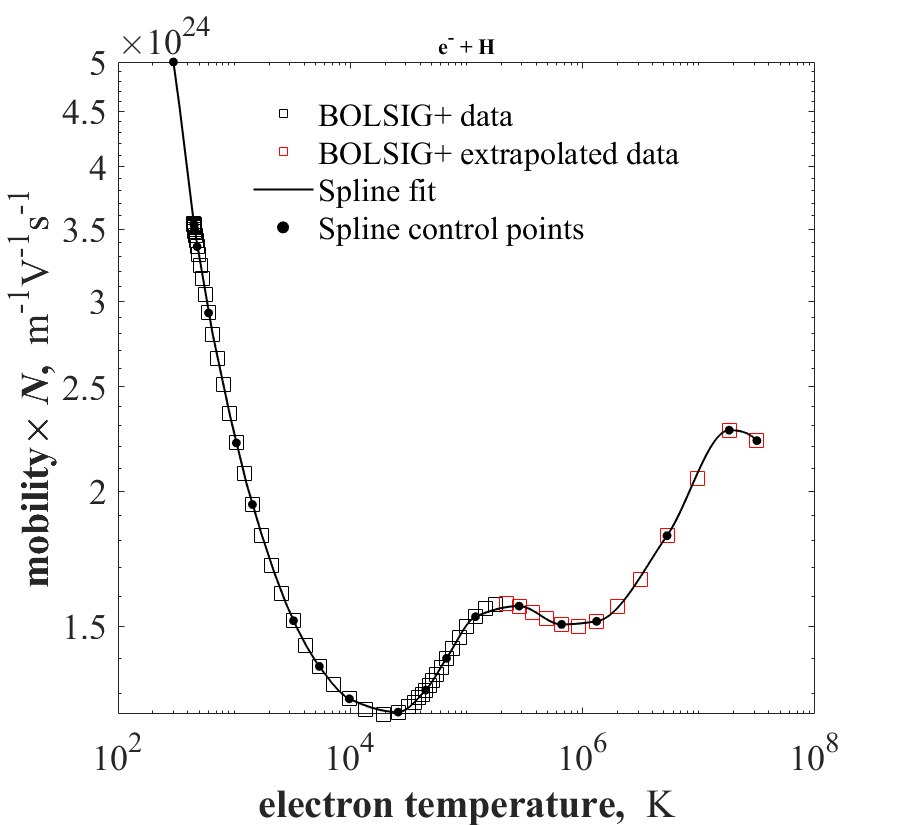
\includegraphics[width=0.99\linewidth, angle=0.0,scale=0.49]{figs/mobility_H.png}}
\subfigure[]{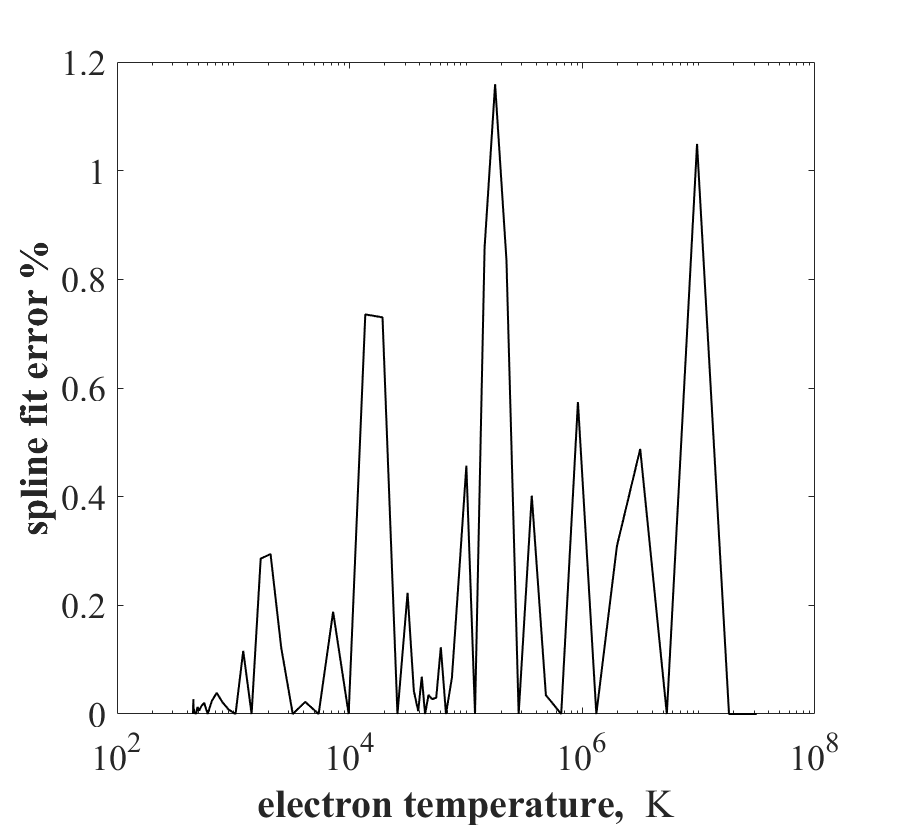
\includegraphics[width=0.99\linewidth, angle=0.0,scale=0.49]{figs/mobility_H_error.png}}
\caption{Results for the mobility of electrons in ${\rm H}$, showing (a) product of mobility and number density, and (b) error percentage of cubic spline fit of  mobility data. The BOLSIG+ calculation uses electron impact cross sections from the Morgan database in Ref.\ \citen{jcp:2012:morgan}.}
\label{fig:mobility_H}
\end{figure}
%
\begin{figure}
\centering
\subfigure[]{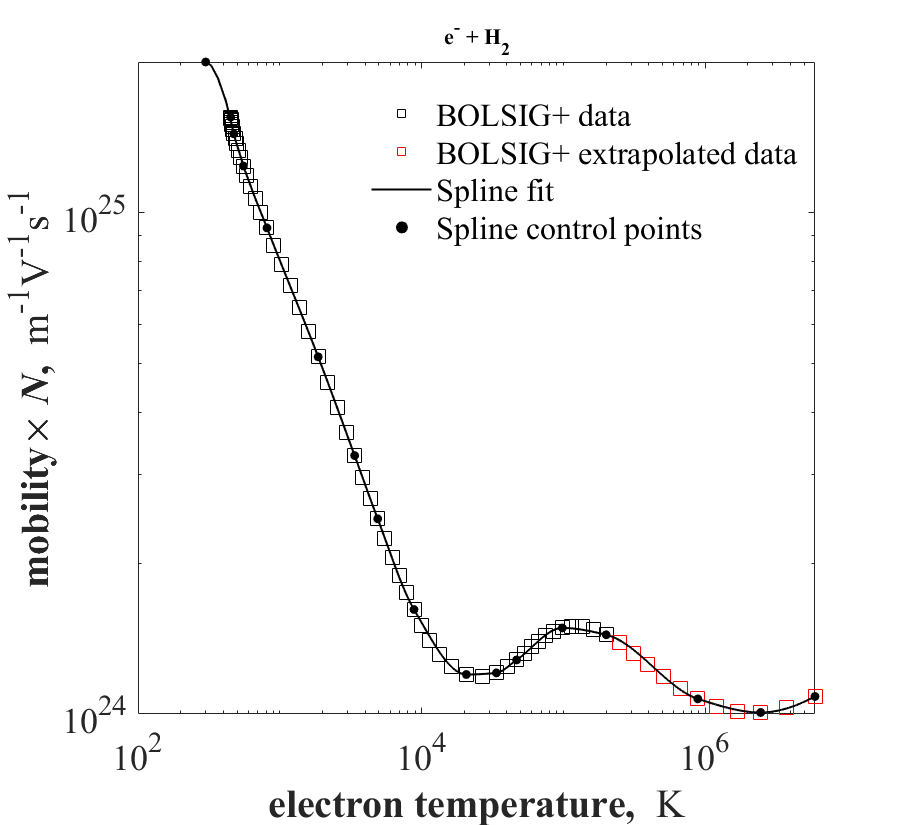
\includegraphics[width=0.99\linewidth, angle=0.0,scale=0.49]{figs/mobility_H2.png}}
\subfigure[]{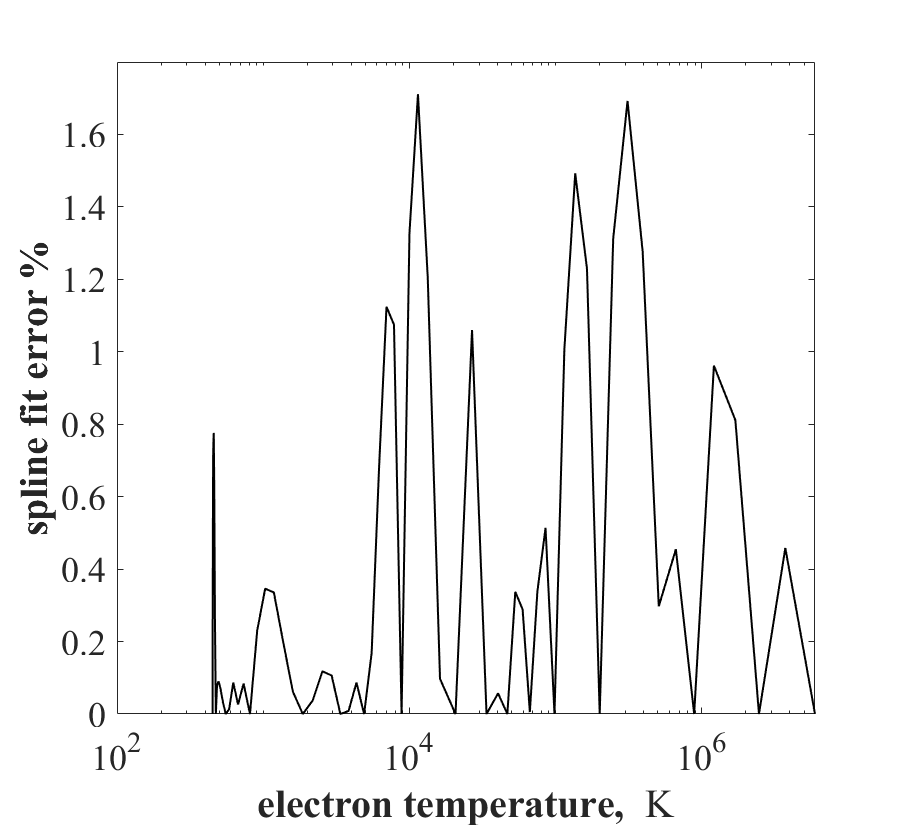
\includegraphics[width=0.99\linewidth, angle=0.0,scale=0.49]{figs/mobility_H2_error.png}}
\caption{Results for the mobility of electrons in ${\rm H_2}$, showing (a) product of mobility and number density, and (b) error percentage of cubic spline fit of  mobility data. The BOLSIG+ calculation uses electron impact cross sections from the Morgan database in Ref.\ \citen{jcp:2012:morgan}.}
\label{fig:mobility_H2}
\end{figure}
%
\begin{figure}
\centering
\subfigure[]{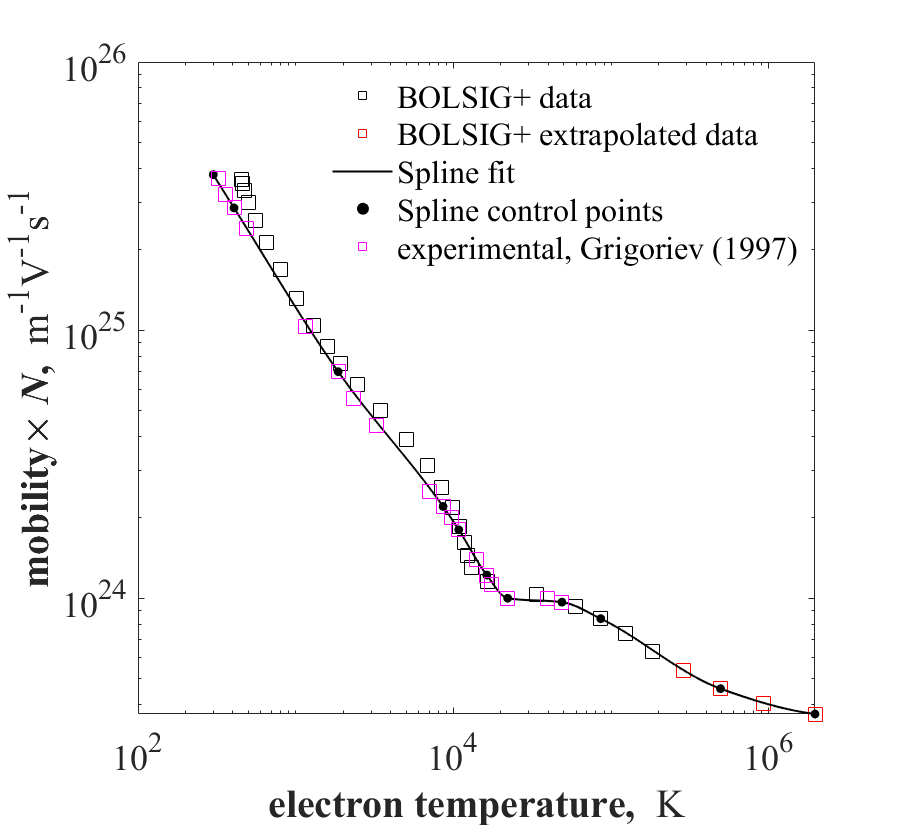
\includegraphics[width=0.99\linewidth, angle=0.0,scale=0.49]{figs/mobility_N2.png}}
\subfigure[]{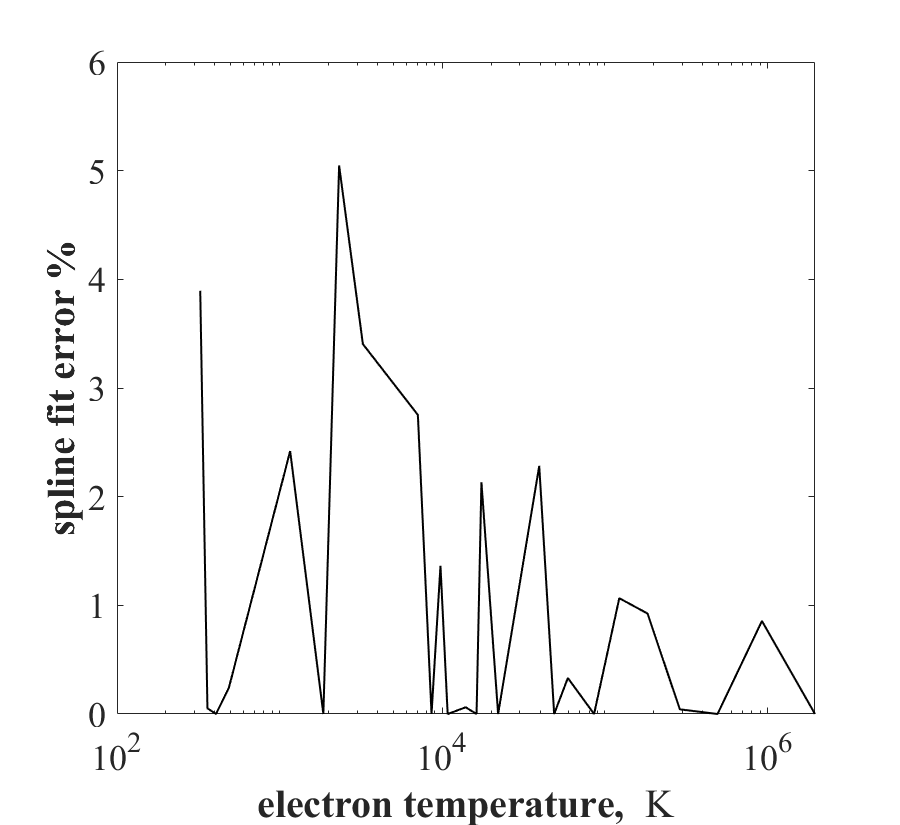
\includegraphics[width=0.99\linewidth, angle=0.0,scale=0.49]{figs/mobility_N2_error.png}}
\caption{Results for the mobility of electrons in ${\rm N_2}$, showing (a) product of mobility and number density, and (b) error percentage of cubic spline fit of  mobility data. The BOLSIG+ calculation uses electron impact cross sections from the Morgan database in Ref.\ \citen{jcp:2012:morgan}. Experimental data obtained from Ch.\ 21 of Ref.\ \citen{book:1997:grigoriev}.}
\label{fig:mobility_N2}
\end{figure}
%
\begin{figure}
\centering
\subfigure[]{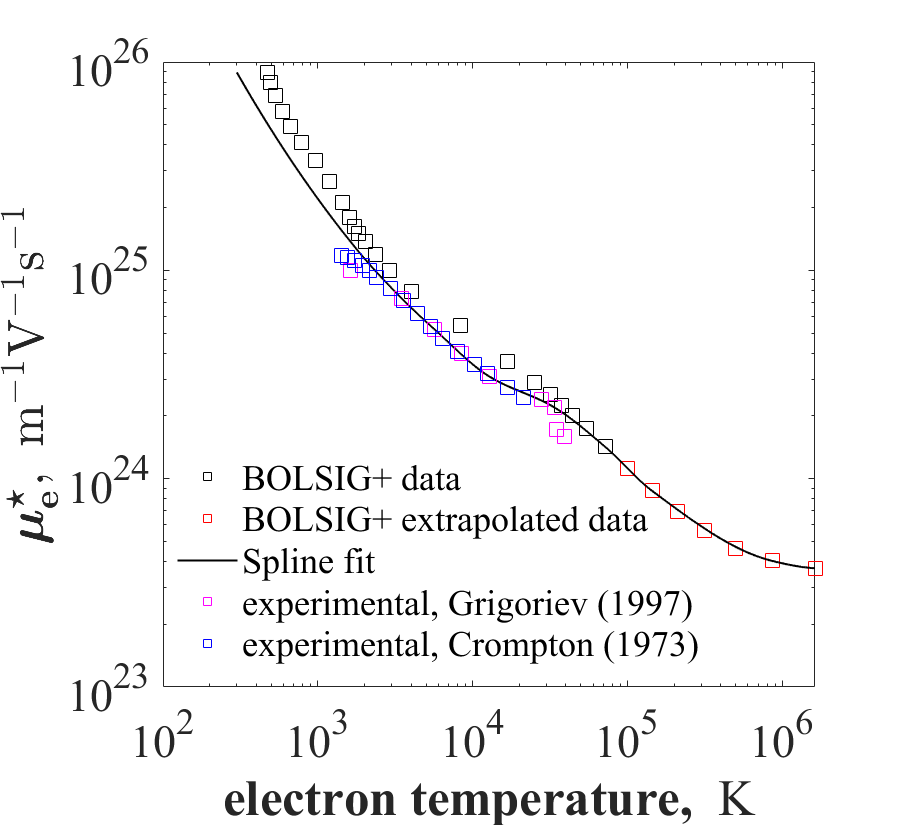
\includegraphics[width=0.99\linewidth, angle=0.0,scale=0.49]{figs/mobility_O2.png}}
\subfigure[]{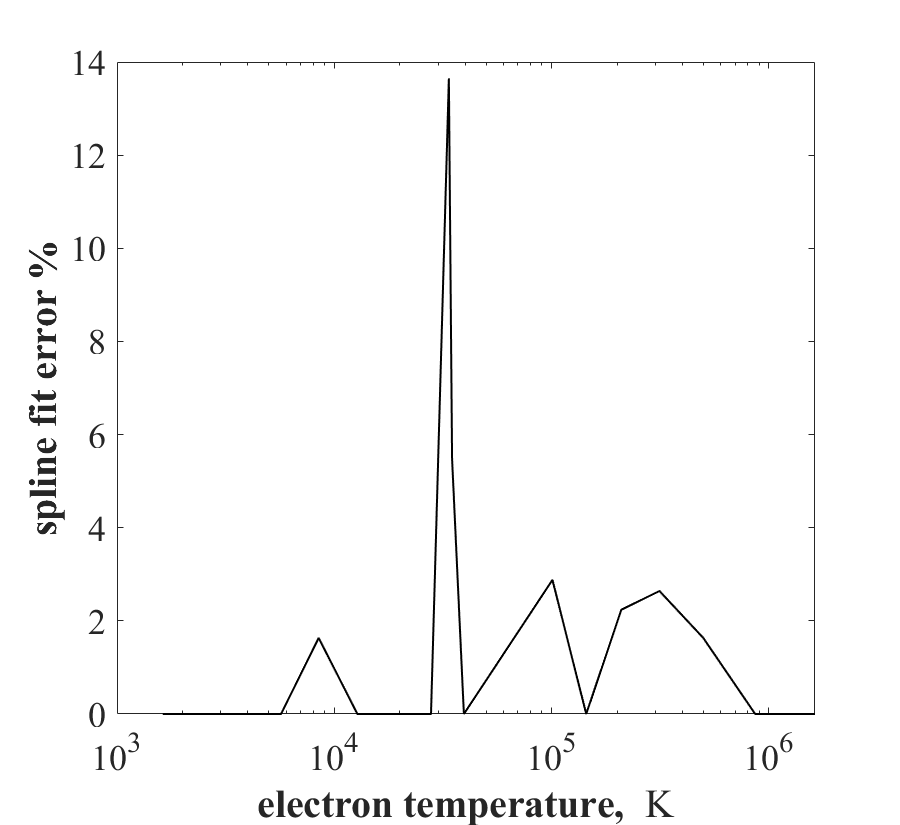
\includegraphics[width=0.99\linewidth, angle=0.0,scale=0.49]{figs/mobility_O2_error.png}}
\caption{Results for the mobility of electrons in ${\rm O_2}$, showing (a) product of mobility and number density, and (b) error percentage of cubic spline fit of  mobility data. The BOLSIG+ calculation uses electron impact cross sections from the Morgan database in Ref.\ \citen{jcp:2012:morgan}. Experimental data obtained from Ch.\ 21 of Ref.\ \citen{book:1997:grigoriev} and Fig. 4 of Ref.\ \citen{ajp:1973:crompton}.}
\label{fig:mobility_O2}
\end{figure}
%
\begin{figure}
\centering
\subfigure[]{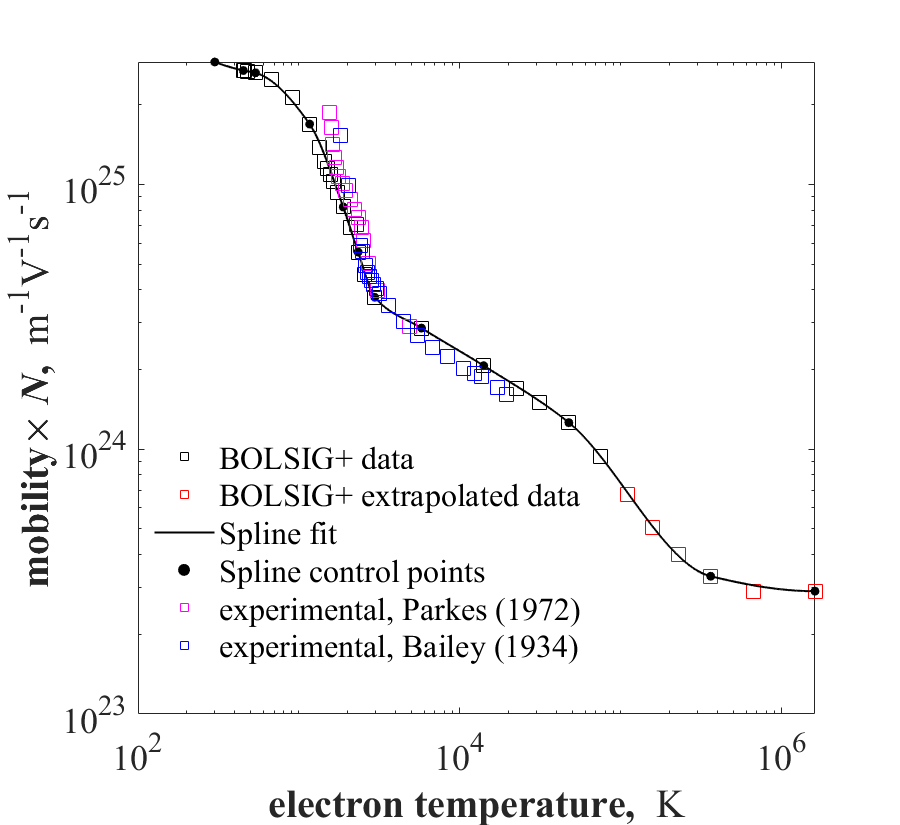
\includegraphics[width=0.99\linewidth, angle=0.0,scale=0.49]{figs/mobility_NO.png}}
\subfigure[]{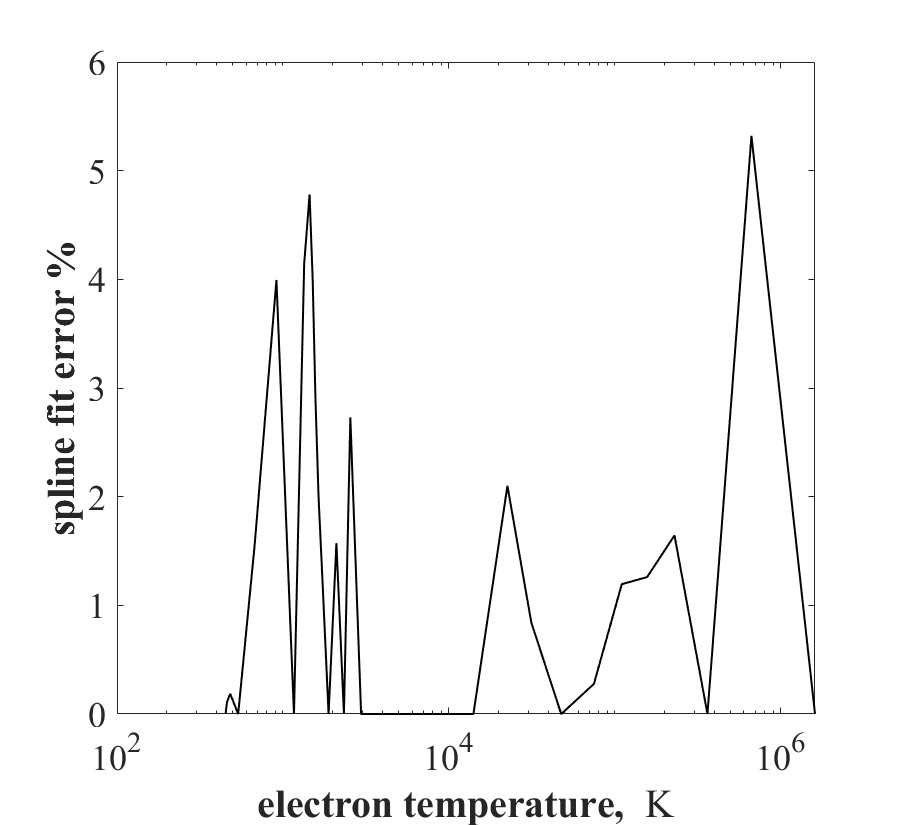
\includegraphics[width=0.99\linewidth, angle=0.0,scale=0.49]{figs/mobility_NO_error.png}}
\caption{Results for the mobility of electrons in ${\rm NO}$, showing (a) product of mobility and number density, and (b) error percentage of cubic spline fit of  mobility data. The BOLSIG+ calculation uses electron impact cross sections from the Phelps database in Ref.\ \citen{jcp:2012:morgan}. Experimental data obtained from Fig.\ 4 of Ref.\ \citen{jos:1934:bailey} and Fig.\ 5 of Ref.\ \citen{jcs:1972:parkes}.}
\label{fig:mobility_NO}
\end{figure}
%
\begin{figure}
\centering
\subfigure[]{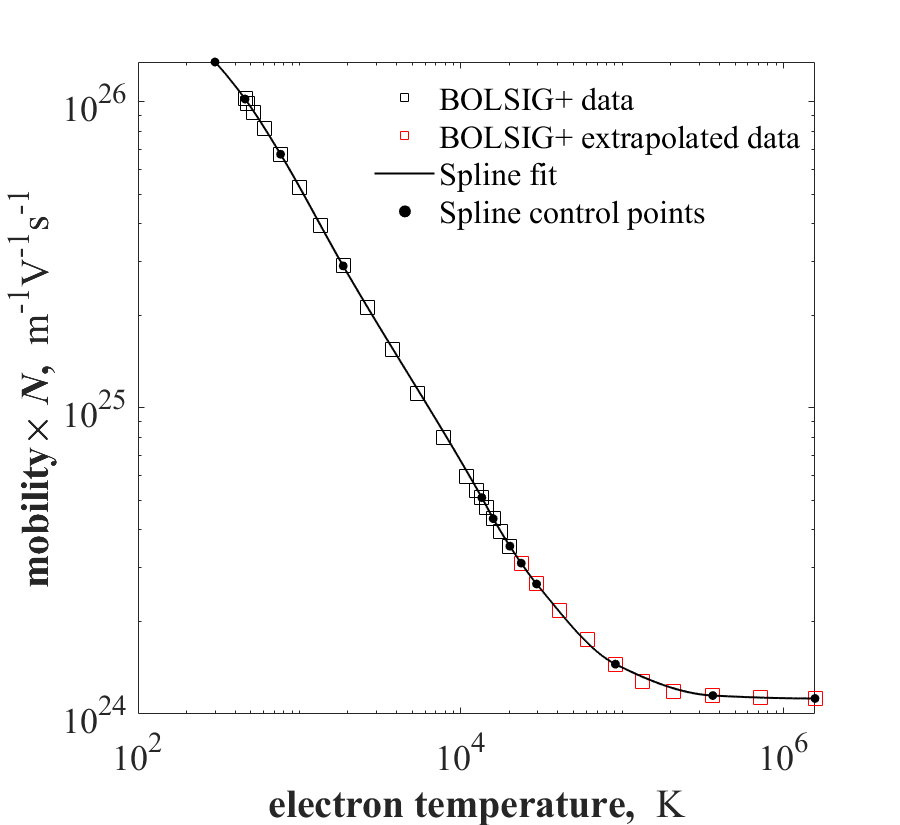
\includegraphics[width=0.99\linewidth, angle=0.0,scale=0.49]{figs/mobility_N.png}}
\subfigure[]{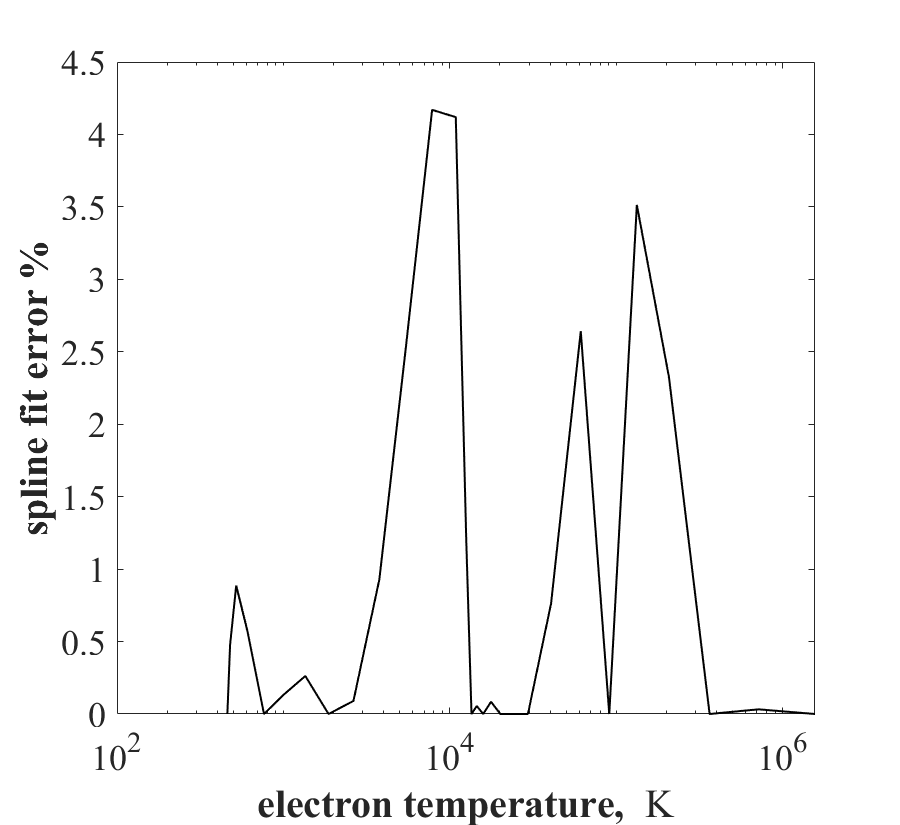
\includegraphics[width=0.99\linewidth, angle=0.0,scale=0.49]{figs/mobility_N_error.png}}
\caption{Results for the mobility of electrons in ${\rm N}$, showing (a) product of mobility and number density, and (b) error percentage of cubic spline fit of  mobility data. The BOLSIG+ calculation uses electron impact cross sections from the Morgan database in Ref.\ \citen{jcp:2012:morgan}.}
\label{fig:mobility_N}
\end{figure}
%
\begin{figure}
\centering
\subfigure[]{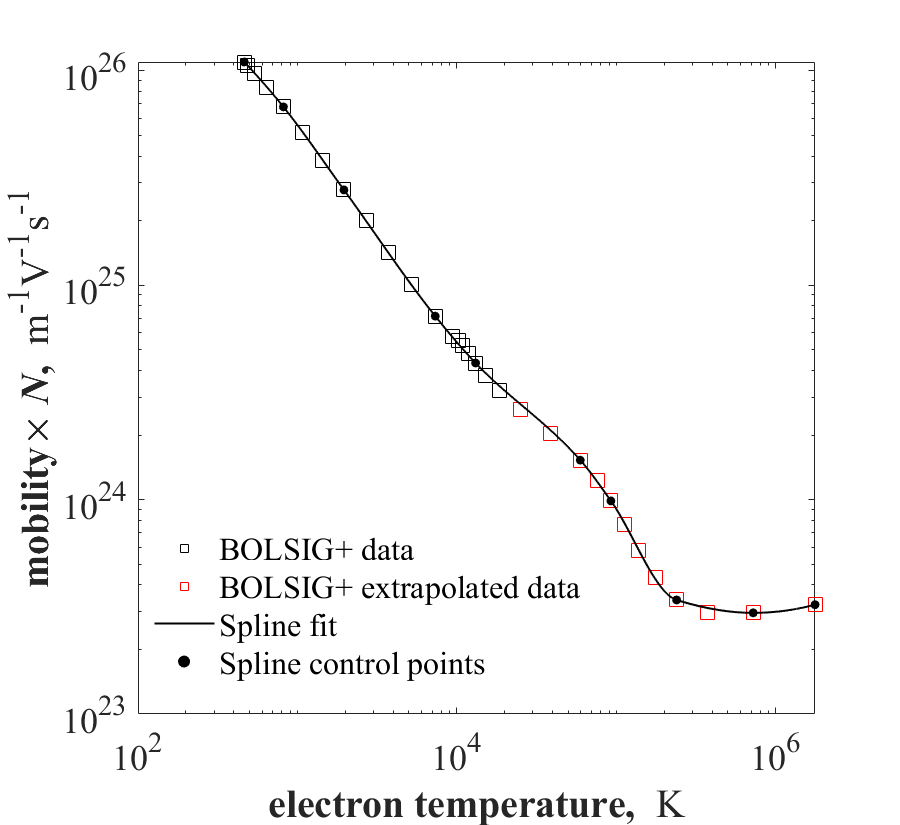
\includegraphics[width=0.99\linewidth, angle=0.0,scale=0.49]{figs/mobility_O.png}}
\subfigure[]{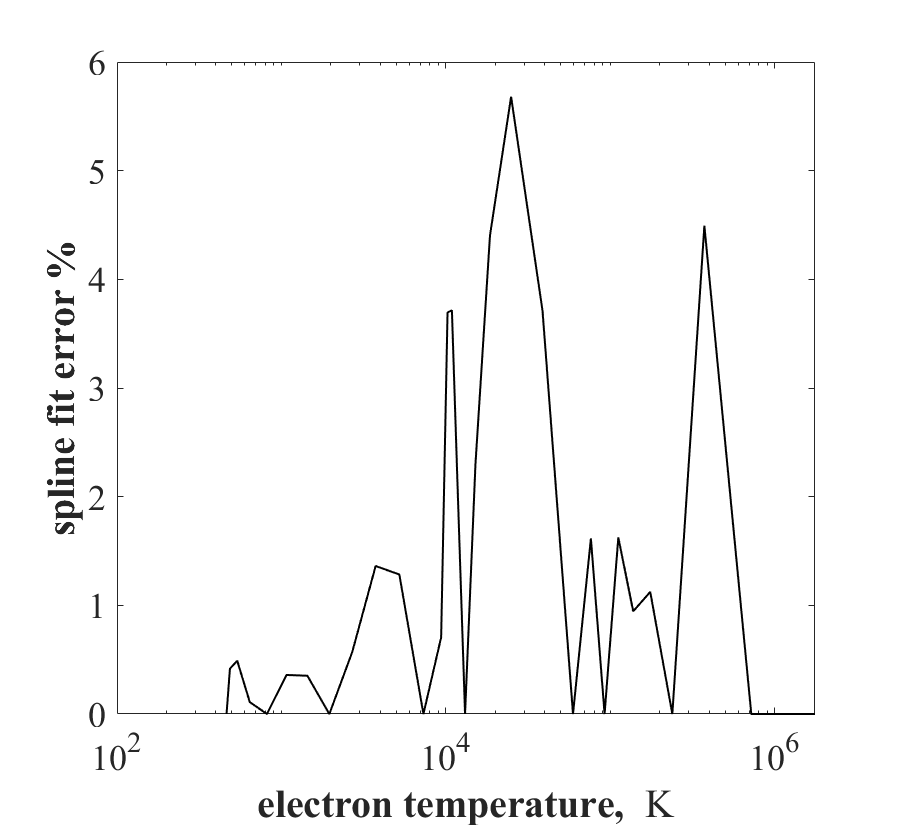
\includegraphics[width=0.99\linewidth, angle=0.0,scale=0.49]{figs/mobility_O_error.png}}
\caption{Results for the mobility of electrons in ${\rm O}$, showing (a) product of mobility and number density, and (b) error percentage of cubic spline fit of  mobility data. The BOLSIG+ calculation uses electron impact cross sections from the Morgan database in Ref.\ \citen{jcp:2012:morgan}.}
\label{fig:mobility_O}
\end{figure}
%
\begin{figure}
\centering
\subfigure[]{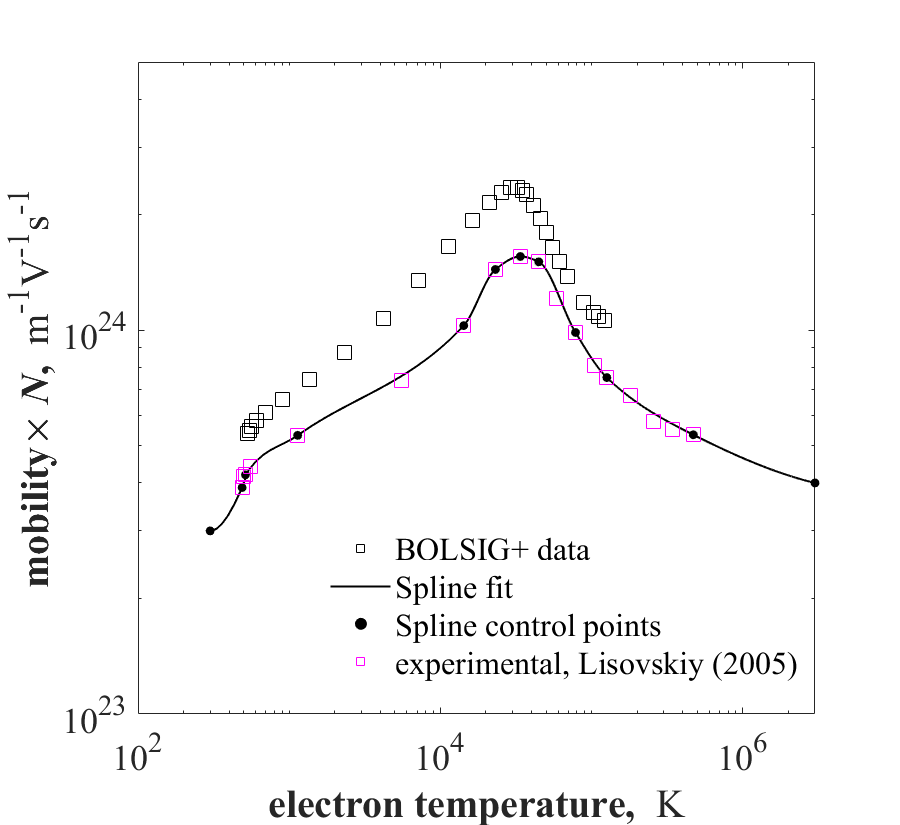
\includegraphics[width=0.99\linewidth, angle=0.0,scale=0.49]{figs/mobility_NH3.png}}
\subfigure[]{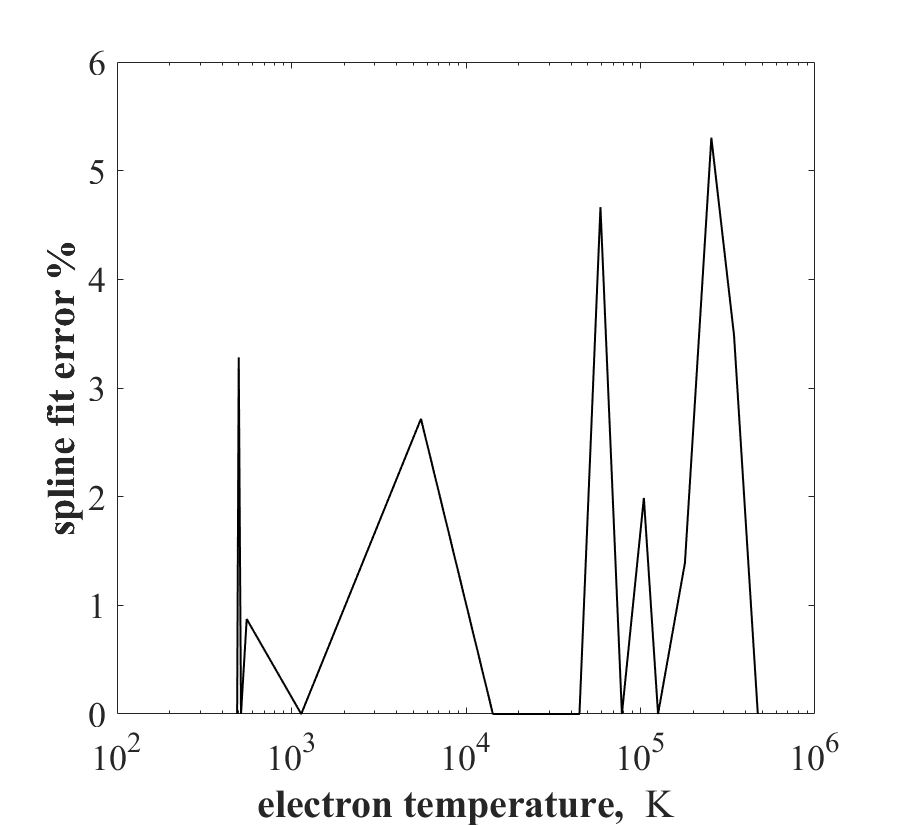
\includegraphics[width=0.99\linewidth, angle=0.0,scale=0.49]{figs/mobility_NH3_error.png}}
\caption{Results for the mobility of electrons in ${\rm NH_3}$, showing (a) product of mobility and number density, and (b) error percentage of cubic spline fit of  mobility data. The BOLSIG+ calculation uses electron impact cross sections from the Morgan database in Ref.\ \citen{jcp:2012:morgan}. Experimental data obtained from Fig.\ 2 of Ref.\ \citen{jopd:2005:lisovskiy}.}
\label{fig:mobility_NH3}
\end{figure}
%
\begin{figure}
\centering
\subfigure[]{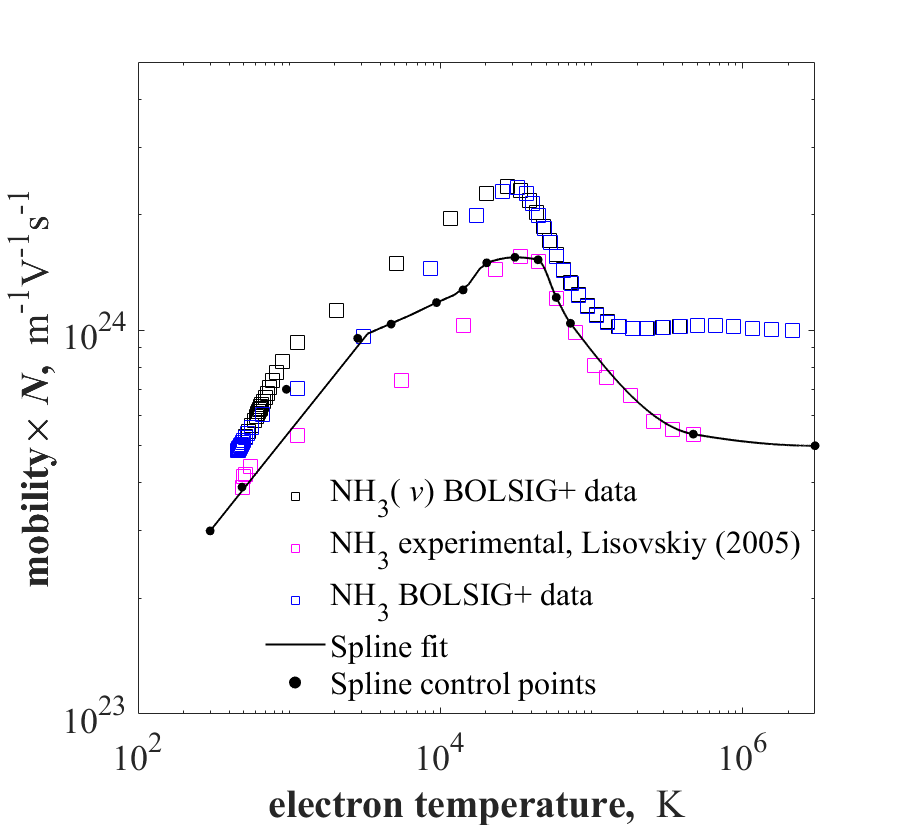
\includegraphics[width=0.99\linewidth, angle=0.0,scale=0.49]{figs/mobility_NH3v.png}}
\subfigure[]{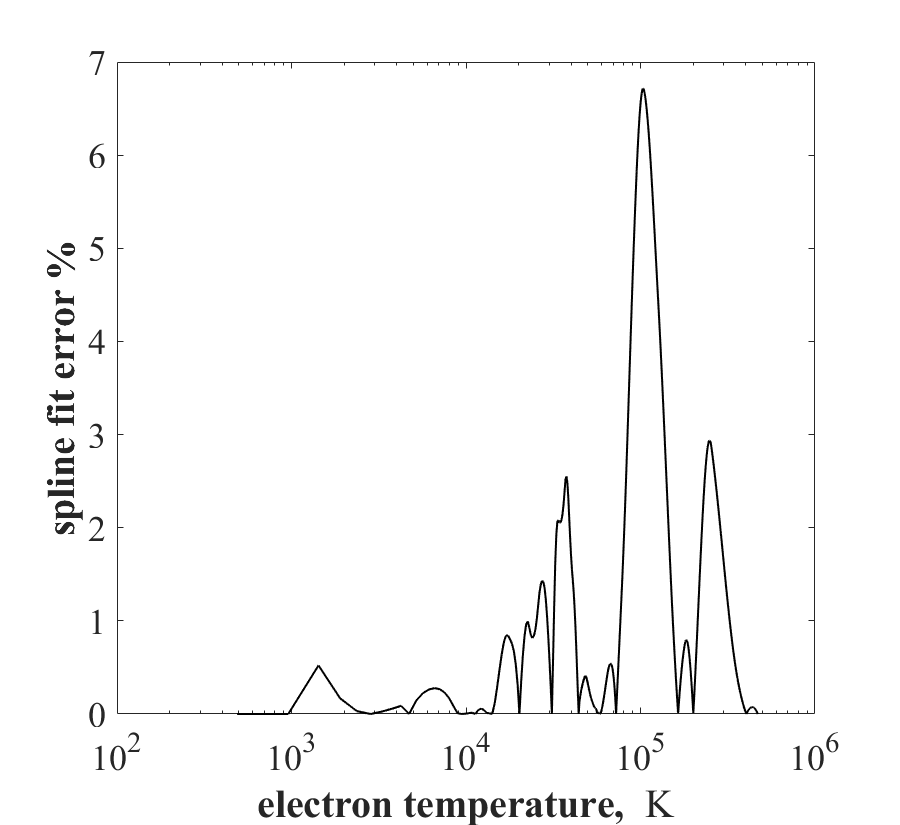
\includegraphics[width=0.99\linewidth, angle=0.0,scale=0.49]{figs/mobility_NH3v_error.png}}
\caption{Results for the mobility of electrons in ${\rm NH_3}$$(v)$, showing (a) product of mobility and number density, and (b) error percentage of cubic spline fit of  mobility data. The BOLSIG+ calculation uses electron impact cross sections from the Morgan database in Ref.\ \citen{jcp:2012:morgan}. Experimental data obtained from Fig.\ 2 of Ref.\ \citen{jopd:2005:lisovskiy}. The final spline is fitted such that the mobility difference between ground state ammonia and ${\rm NH_3}$$(v)$ is added to the experimental ${\rm NH_3}$ mobility data set.}
\label{fig:mobility_NH3v}
\end{figure}
%
\begin{figure}
\centering
\subfigure[]{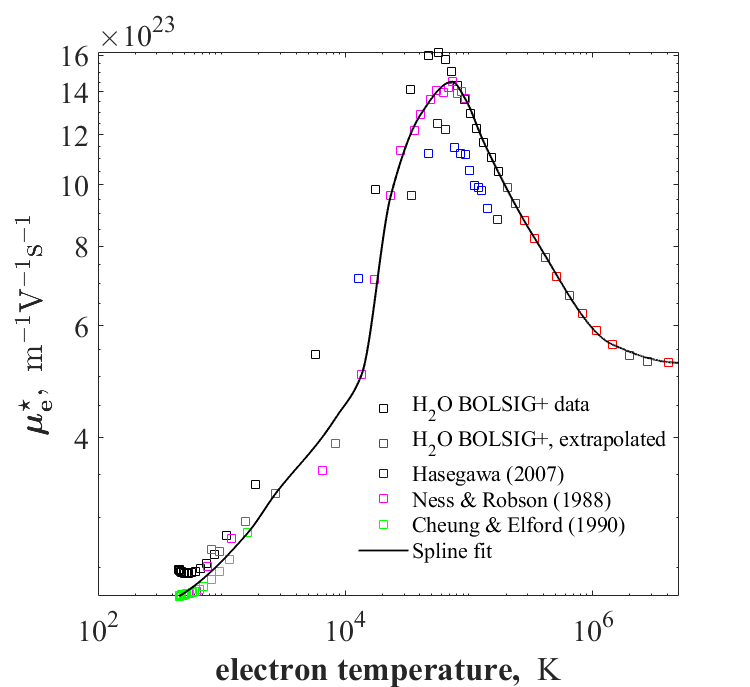
\includegraphics[width=0.99\linewidth, angle=0.0,scale=0.49]{figs/mobility_H2O.png}}
\caption{Results for the mobility of electrons in ${\rm H_2O}$, showing (a) product of mobility and number density, and (b) error percentage of cubic spline fit of  mobility data. The BOLSIG+ calculation uses electron impact cross sections from the TRINITI database with cross-sections from Ref.\ \citen{phig:1987:yousfi}. Experimental data points are taken from Fig. 1. of Ref.\ \cite{jop:2007:hasegawa}, Fig. 4 of Ref.\ \cite{pra:1988:ness} and Table 1 of Ref.\ \cite{ajp:1990:cheung}.}
\label{fig:mobility_H2O}
\end{figure}
%
\begin{figure}
\centering
\subfigure[]{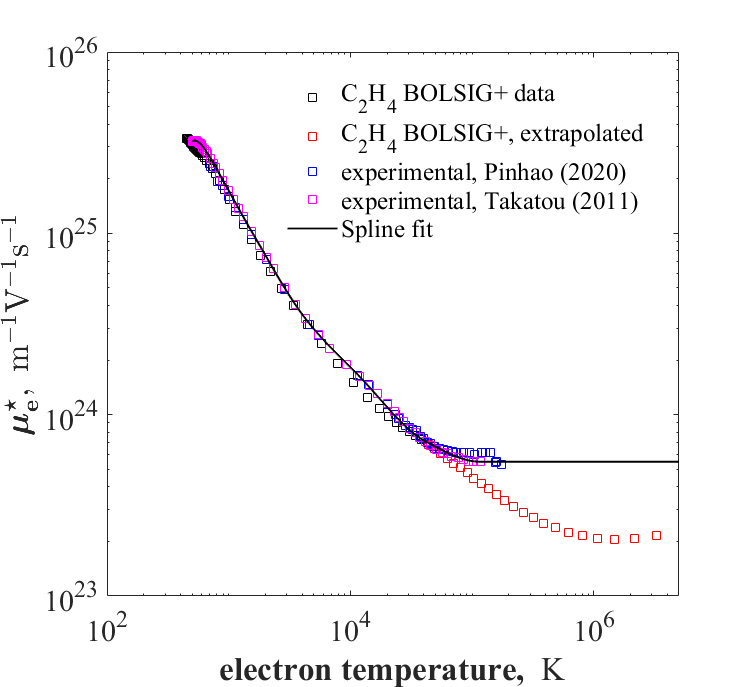
\includegraphics[width=0.99\linewidth, angle=0.0,scale=0.49]{figs/mobility_C2H4.png}}
\caption{Results for the mobility of electrons in ${\rm C_2H_4}$, showing (a) product of mobility and number density, and (b) error percentage of cubic spline fit of  mobility data. The BOLSIG+ calculation uses electron impact cross sections from the TRINITI database with cross-sections from Ref.\ \citen{phig:1987:yousfi}. Experimental data points are taken from Fig. 4 of Ref.\ \cite{jop:2011:takatou} and Fig. 5 of Ref.\ \cite{psst:2020:pinhao}.}
\label{fig:mobility_C2H4}
\end{figure}
%
\begin{figure}
\centering
\subfigure[]{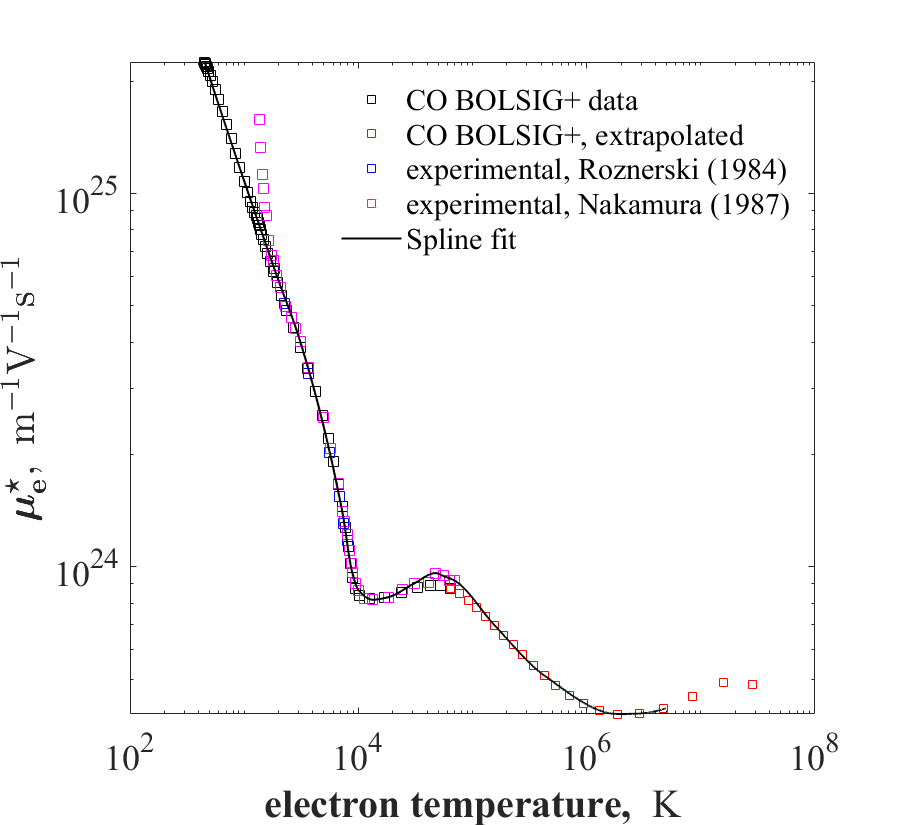
\includegraphics[width=0.99\linewidth, angle=0.0,scale=0.49]{figs/mobility_CO.png}}
\caption{Results for the mobility of electrons in ${\rm CO}$, showing (a) product of mobility and number density, and (b) error percentage of cubic spline fit of  mobility data. The BOLSIG+ calculation uses electron impact cross sections from the lxcat Morgan database. Experimental data points are taken from Fig. 6 of Ref.\ \cite{jop:1987:nakamura} and Fig. 3 of Ref.\ \cite{jop:1984:roznerski}.}
\label{fig:mobility_CO}
\end{figure}

\subsection{Electron Mobility}

The electron mobility in a partially ionized plasma (a plasma in which both the molar fraction of all neutrals and the molar fraction of all charged species are significant) needs to include collisions between the electrons and the neutrals and collisions between electrons and ions. This results in an electron mobility equal to:
%
\begin{equation}
\mu_{\rm e}=\frac{1}{\mfd \sum_k^{k\ne e} \frac{N_k}{\mu_{{\rm e}k}N_k}}
\end{equation}
%
or
%
\begin{equation}
\mu_{\rm e} N=\frac{1}{\mfd \sum_k^{k\ne e} \frac{\chi_k}{\mu_{{\rm e}k}N_k}}
\end{equation}
%
with $\chi_k$ the molar fraction of species $k$, $N$ the total number density of the mixture (including electrons), and $N_k$ the number density of species $k$, and $\mu_{{\rm e}k}$ the mobility of the electrons within species $k$. 




We can rewrite the collision frequency between the electrons and species $k$,  $\nu_{\rm ek}$, as function of the mobility \cite[page 9]{book:1991:raizer} or the collision cross section as follows:
%
\begin{equation}
\nu_{ek} = \frac{|C_{\rm e}|}{m_{\rm e} \mu_{ek}} = N_k \sigma_{ek} \overline{q_{\rm e}} 
\end{equation}
%
where $\mu_{ek}$ is the electron mobility within species $k$ and where  $\sigma_{ek}$ is the collision cross section between an electron and species $k$ and $\overline{q_{\rm e}}$ is the average electron speed.  We can use the latter to express the electron mobility within species $k$ as a function of the collision cross-section $\sigma_{ek}$ as follows:
%
\begin{equation}
\mu_{ek}N_k = \frac{|C_{\rm e}|}{m_{\rm e} \sigma_{ek} \overline{q_{\rm e}}}   
\end{equation}
%
We can further express  $\sigma_{ek}$ following Ref.~\cite[page 58]{book:2004:lieberman}:
%
\begin{equation}
\sigma_{ek}= \frac{8}{\pi} b_0^2 \ln \Lambda
\end{equation}
%
with $\ln \Lambda$ the Coulomb logarithm and $b_0$ equal to \cite[page 56]{book:2004:lieberman}:
%
\begin{equation}
b_0 = \frac{|C_k| |C_e|}{4 \pi \epsilon_0 } \frac{1}{\frac{1}{2} m_{\rm e} \overline{q_{\rm e}}^2}
\end{equation}
%
Then 
%
\begin{equation}
\mu_{ek}N_k = \frac{|C_{\rm e}|}{m_{\rm e} \frac{8}{\pi} \left(\frac{|C_k| |C_e|}{4 \pi \epsilon_0 } \frac{1}{\frac{1}{2} m_{\rm e} \overline{q_{\rm e}}^2} \right)^2 \ln \Lambda \overline{q_{\rm e}}}   
\end{equation}
%
or
%
\begin{equation}
\mu_{ek}N_k = \frac{ \pi^3 \epsilon_0^2 m_{\rm e} \overline{q_{\rm e}}^3}{ 2  C_k^2 |C_e| \ln \Lambda }   
\end{equation}
%
In the latter $\overline{q_{\rm e}}$ is the average speed of the electrons approaching an ion:
%
\begin{equation}
\overline{q_{\rm e}} = \sqrt{\frac{8 k_{\rm B} T_{\rm e}}{\pi m_{\rm e}}}
\end{equation}
%
Substitute:
%
\begin{equation}
\mu_{ek}N_k = \frac{ \pi^3 \epsilon_0^2 m_{\rm e}}{ 2  C_k^2 |C_e| \ln \Lambda } 
\left(\frac{8 k_{\rm B} }{\pi m_{\rm e}}\right)^\frac{3}{2} T_{\rm e}^{1.5} {\rm ~~~when~kth~species~is~ionic}
\end{equation}
%
Another way we can obtain the electron mobility within a ionic species is by starting from Raizer \cite[Eq.\ (2.9)]{book:1991:raizer}:
%
\begin{equation}
\mu_{{\rm e}k} N_k= \frac{9.5 \times 10^{16}}{\rm m\cdot K^{1.5}\cdot V \cdot s} \frac{T_{\rm e}^{1.5}}{ \ln \Lambda} {\rm ~~~when~kth~species~is~ionic}
\end{equation}
%
where $T_{\rm e}$ is the electron temperature in K, $N_{k}$ is the $k$th ion number density in m$^{-3}$.
The latter two expressions for the electron mobility within an ionic gas differ only by a constant of proportionality as follows:
%
\begin{equation}
\mu_{ek}N_k = \frac{1.47 \cdot \pi^3 \epsilon_0^2 m_{\rm e}}{ 2  C_k^2 |C_e| \ln \Lambda } 
\left(\frac{8 k_{\rm B} }{\pi m_{\rm e}}\right)^\frac{3}{2} T_{\rm e}^{1.5} {\rm ~~~when~kth~species~is~ionic}
\end{equation}
%


Also, $\Lambda$ is the shielding parameter and $\ln \Lambda$ is the Coulomb logarithm. The Coulomb logarithm can be  found from the following \cite[p. 14]{book:1991:raizer}:
%
\begin{equation}
    \ln \Lambda=13.57+\frac{3}{2} {\rm log}_{10} \left(\frac{T_{\rm e}}{11600}\right)-\frac{1}{2}{\rm log}_{10}\left(\frac{N_{\rm e}}{10^6}\right)
\end{equation}
%
with $\rho_{\rm e}$ the electron partial density in kg/m$^3$, $m_{\rm e}$ the electron mass in kg, $N_{\rm e}$ the electron number density in m$^{-3}$, and $T_{\rm e}$ the electron temperature in K.

However, we find that using the latter leads to the electrical conductivity being underestimated by 30\% for equilibrium air or equilibrium hydrogen plasmas (see experimental data of electrical conductivity on \cite[page 276]{book:1991:raizer}). We get better agreement with experimental data by using the Coulomb logarithm recommended in the NRL Plasma Formulary for electron-ion collisions \cite[page 34]{nrl:2002:huba}:
%
\begin{equation}
 \ln \Lambda = 23-\ln \left(\left(N_{\rm e}/1e6\right)^\frac{1}{2} \cdot (T_{\rm e}/11600.0)^{-1.5}\right)
\end{equation}
%
with $N_{\rm e}$ the electron number density in 1/m$^3$ and $T_{\rm e}$ the electron temperature in K. The latter is valid as long as the electron temperature is less than 10 eV. 


A first approximation for the mobility of electrons within a neutral gas can be obtained from the experimental data of electron mobility in air outlined in in Chapter 21 of Ref.\ \cite{book:1997:grigoriev} (in units of $\rm m^2\cdot V^{-1}\cdot s^{-1}$):
%
\begin{equation}
\mu_{{\rm e}k} N_k= 3.74\cdot 10^{19} \cdot {\rm exp}\left(33.5 \cdot \left({\rm ln}\, T_{\rm e} \right)^{-0.5}\right) {\rm ~~~when~kth~species~is~neutral}
\end{equation}
%
where $N_k$ is the number density of species $k$ in $m^{-3}$ and $T_{\rm e}$ is the electron temperature in K.
The latter equation can be used in the range $1000~{\rm K} \le T_{\rm e} \le 57900 ~{\rm K}$ with a relative error on the mobility not exceeding 20\%. In the range $287~{\rm K} \le T_{\rm e} < 1000~{\rm K}$, the relative error is less than 30\%. 

A better evaluation of the mobility within a neutral gas can be obtained from BOLSIG+ as follows:
%
\begin{equation}
\mu_{{\rm e}k} N_k = (\mu_{{\rm e}k} N)(T_{\rm e}) {\rm ~~~when~kth~species~is~neutral}
\end{equation}
%
where $(\mu_{{\rm e}k} N)(T_{\rm e})$ refers to $\mu_{{\rm e}k} N$ as a function of $T_{\rm e}$ for a species $k$ obtained from BOLSIG+ or from the drift velocity measured experimentally as shown in Table \ref{tab:electrondriftvelocities} for N$_2$, O$_2$ and Air.


\subsection{Ion Mobility}

When the plasma has a low ionization fraction, the ion mobility depends only on ion-neutral collisions. When the plasma's ionization fraction increases, then the ion-ion collisions can also affect the mobility. We thus formulate the ion mobility as follows:
%
\begin{equation}
\mu_{\rm i}=\frac{1}{\frac{1}{\mu_{\rm in}}+\frac{1}{\mu_{\rm ii}}}
\end{equation}
%
where $\mu_{\rm ii}$ is the ion mobility in the limit of a fully ionized plasma and $\mu_{\rm in}$ is the ion mobility in the limit of a weakly-ionized plasma. The ion mobility for a fully ionized plasma is found from the collision frequency of ion-ion collisions as follows:
%
\begin{equation}
 \mu_{\rm ii} = \frac{|C_i|}{m_i \nu_{\rm ii}}
\end{equation}
% 
where $C_i$ is the charge of the ion in Coulomb and where the ion-ion collision frequency corresponds to \cite{book:1984:chen}:
%
\begin{equation}
\nu_{\rm ii}=\xi \frac{ N_{\rm i}}{ \sqrt{m_{\rm i}} (k_{\rm B} T_{\rm i})^\frac{3}{2}}  \frac{C_{\rm i}^4}{16 \pi^2 \epsilon_0^2}  \ln \Lambda
\end{equation}
%
with $\xi$ a non-dimensional constant in the range 1.7-2.4. As well, $\ln \Lambda$ is another constant in the range 5-7.


After substituting the latter in the former:
%
\begin{equation}
 \mu_{\rm ii} = \frac{16 \pi^2 \epsilon_0^2 (k_{\rm B} T_{\rm i})^\frac{3}{2}}{\mfd \sqrt{m_{\rm i}} \xi  N_{\rm i}  |C_{\rm i}|^3  \ln \Lambda}
\end{equation}
% 
Setting $\xi$ to 1.71 and $\ln \Lambda$ to 6.3, and assuming that the ion has a single charge, the latter can be rewritten as:
%
\begin{equation}
 \mu_{\rm ii} = 14.3 m_{\rm i}^{-0.5} T_{\rm i}^{1.5} N_{\rm i}^{-1}
\end{equation}
% 
where $m_{\rm i}$ is the ion mass in kg, $T_{\rm i}$ the ion translational temperature in K, $N_{\rm i}$ the total ion number density in $\rm m^{-3}$, and $\mu_{\rm i}$ the ion mobility in m$^2$/Vs.


We can find the ion mobility for a weakly-ionized plasma $\mu_{\rm in}$ through the collision frequency between ions and neutrals. For instance, for the nitrogen ion $\rm N_2^+$, the mobility in air can be expressed as:
%
\begin{equation}
\mu_{\rm in}=N_{\rm n}^{-1} \cdot 0.75\cdot 10^{23}\cdot T^{-0.5}
\end{equation}
%
where $N_{\rm n}$ is the number density of the neutrals in $m^{-3}$ and $T$ is the ion translational temperature in K, and $\mu_{\rm in}$ is the ion mobility in a weakly-ionized plasma in m$^2$/V-s.

The mobility of a partially-ionized plasma (in-between weakly-ionized and fully-ionized) can be obtained simply by taking half of the harmonic mean of the mobility of a fully-ionized plasma and the mobility of a weakly-ionized plasma. 

The ion mobilities of the various charged species are tabulated in Table \ref{tab:pm:mu}. 



\subsection{Electron and Ion Thermal Conductivity}

Whether the plasma is fully-ionized or weakly-ionized, the thermal conductivity can be expressed as a function of the mobility as follows:
%
\begin{equation}
\kappa_k =     \frac{ \rho_k k_{\rm B}  (c_p)_k T_k \mu_k}{|C_k|} 
\end{equation}
%
where $(c_p)_k$ is the specific heat at constant pressure of the $k$th species.

\subsection{Electron and Ion Viscosity}

The scalar viscosity can be obtained from the thermal conductivity as follows:
%
\begin{equation}
\eta_k = \frac{{\rm Pr} \cdot \kappa_k}{(c_p)_k}
\end{equation}
% 
where Pr is the Prandtl number which is set to 0.73 for the electrons and to 0.96 for the ions.

\subsection{Diffusion Coefficient}

The diffusion coefficient ${\cal D}$ is related to the mobility $\mu$ following the Einsteins-Smoluchowski relation as follows:
%
\begin{equation}
    {\cal D}_k= \frac{\mu_k k_{\rm B} T_k}{|C_k|}
\end{equation}
%
with $\mu_k$ the mobility in m$^2$/V-s, $\cal D$ the diffusion coefficient in m$^2$/s, $C_k$ the charge in Coulomb of one particule and $k_{\rm B}$ the Boltzmann constant.




\section{Dixon-Lewis Transport Coefficients}
%
\begin{table}[t]
\fontsizetable
\begin{center}
  \begin{threeparttable}
    \tablecaption{$\epsilon$ and $\sigma$ for some species \tnote{1}}
    \fontsizetable
    \begin{tabular}{lllll}
      \toprule
species$_k$     &  ${\rm He}$    &  ${\rm H}_2$   &  ${\rm O}_2$   &  ${\rm N}_2$  \\
\midrule
$\epsilon_k$ [K]&  $10.22$       &  $59.7$        &  $106.7$       &  $71.4$       \\
$\sigma_k$ [nm] &  $0.2576$      &  $0.2827$      &  $0.3467$      &  $0.3798$     \\
      \bottomrule
    \end{tabular}
    \label{tab:dl:epsilon-sigma}
    \begin{tablenotes}
      \item [1] taken from Dixon-Lewis; $T^\star_k=T/ \epsilon_k$
    \end{tablenotes}
  \end{threeparttable}
\end{center}
\end{table}
%
%
\begin{table*}[t]
\fontsizetable
\begin{center}
  \begin{threeparttable}
    \tablecaption{Polynomial constants needed to determine $\Omega^{22}$ 
             $\Omega^{11}$ and $A^\star$ taken from Dixon-Lewis}
    \fontsizetable
    \begin{tabular*}{\textwidth}{@{\extracolsep{\fill}}llllll}
      \toprule
$T^\star_k$& $d_0$          & $d_1$           & $d_2$          & $d_3$           & $d_4$ \\
\midrule
$<5$       & $2.3527333$E$+0$ & $-1.3589968$E$+0$ & $5.2202460$E$-1$ & $-9.4262883$E$-2$ & $6.4354629$E$-3$ \\
$5-10$     & $1.2660308$E$+0$ & $-1.6441443$E$-1$ & $2.2945928$E$-2$ & $-1.6324168$E$-3$ & $4.5833672$E$-5$ \\
$>10$      & $8.5263337$E$-1$ & $-1.3552911$E$-2$ & $2.6162080$E$-4$ & $-2.4647654$E$-6$ & $8.6538568$E$-9$ \\
\midrule
$T^\star_k$& $e_0$          & $e_1$           & $e_2$           &~&~\\
\midrule
$<5$       & $1.1077725$E$+0$ & $-9.4802344$E$-3$ & $+1.6918277$E$-3$ &~&~ \\
$5-10$     & $1.0871429$E$+0$ & $+3.1964282$E$-3$ & $-8.9285689$E$-5$ &~& ~\\
$>10$      & $1.1059000$E$+0$ & $+6.5136364$E$-4$ & $-3.4090910$E$-6$ &~&~ \\
      \bottomrule
    \end{tabular*}
    \label{tab:dl:Omega}
    \begin{tablenotes}
      \item  $\Omega^{22}(T^\star_k)= A^\star (T^\star_k) \Omega^{11}(T^\star_k)$ 
      \item  $\Omega^{11}(T^\star_k)=d_0+d_1 {T^\star_k}+d_2 {T^\star_k}^2+d_3 {T^\star_k}^3+d_4 {T^\star_k}^4$ 
      \item  $A^\star (T^\star_k)=e_0+e_1 {T^\star_k}+e_2 {T^\star_k}^2$ 
    \end{tablenotes}
  \end{threeparttable}
\end{center}
\end{table*}
%

\subsection{Neutrals Mixture Viscosity}

The viscosity of the mixture of neutral gases $\eta_{\rm n}$ is computed using Wilke's mixing rule:
%
\begin{equation}
\eta_{\rm n}= \mfd \chi_{\rm n} \sum_{\mfa k=1}^{\ns}   \frac{\mfd \eta_k {\chi}_k^\star}
                     {\mfd {\chi}_k^\star +
                          \mfd\sum_{\mfa l=1..\ns}^{l \neq k}{\chi}_l^\star \phi_{k,l}}
\label{eqn:dl:molvisc-mixture}
\end{equation}
%
where $\chi_k^\star$ is the neutral molar fraction. That is, $\chi_k^\star$ is the ratio between the number of moles of species $k$ and the number of moles of all neutral species:
%
\begin{equation}
  \chi_k^\star
  = \frac{N_k}{\mfd\sum_{j=1..\ns}^{j \neq {\rm e,i}} N_j} = \frac{\rho_k/m_k}{\mfd\sum_{j=1..\ns}^{j \neq {\rm e,i}} \rho_j/m_j} 
= \frac{w_k /m_k}{\mfd\sum_{j=1..\ns}^{j \neq {\rm e,i}} w_j /m_j} 
\end{equation}
%
where $m_k$ is the particule mass of the $k$th species and $N_k$ is the number density of the $k$th species. Also, $\chi_{\rm n}$ is the molar fraction of the neutrals within the mixture:
%
\begin{equation}
    \chi_{\rm n}= \frac{\mfd \sum_{k=1..\ns}^{k\neq {\rm i,e}} N_k }{\mfd \sum_{k=1}^\ns N_k}
    =\frac{\mfd \sum_{k=1..\ns}^{k\neq {\rm i,e}} \frac{w_k}{m_k} }{\mfd \sum_{k=1}^\ns \frac{w_k}{m_k}}
\end{equation}



Also $\phi_{k,l}$ is specified as follows:
%
\begin{equation}
\phi_{k,l}=\mfd \frac{ \left[  1 + \sqrt{ \mfd {\eta_k }/{\eta_l }}
                              \left( \mfd {{\cal M}_l}/{{\cal M}_k}  \right)^ \frac{1}{4}  \right]^2}
{ \sqrt{\mfd 8\left(1+\mfd {{\cal M}_k}/{{\cal M}_l}\right)}}
\label{eqn:dl:molvisc-phi}
\end{equation}
%
where $\cal M_k$ is the molecular weight of the $k$th species.

Also, the species dynamic viscosity $\eta_k$ in kg/m-s is
derived from kinetic theory assuming that species $k$ is a pure gas (standalone, not mixed with other species):
%
\begin{equation}
\eta_k= 
\mfd 8.44107 \cdot 10^{-7} \cdot \frac{  \sqrt{{\cal M}_k T}}{\sigma_k^2 \Omega^{22}_k} 
\label{eqn:dl:molvisc-muk1}
\end{equation}
%
In the latter ${\cal M}_k$ is the molecular weight in kg/mole and $m_k$ is the mass of one electron or ion in kg.  Also $\sigma_k$ is the Lennard-Jones collision diameter tabulated in Table \ref{tab:dl:epsilon-sigma} in nm. 
Further, $\Omega^{22}_k$ is the reduced collision integral involving polynomials function of $T^\star_k$ with  $T^\star_k$
 is the non-dimensional reduced temperature corresponding to $T/ \epsilon_k$  with $\epsilon_k$ being the Lennard-Jones potential well depth in Kelvin. Data for $\epsilon_k$ can be found in Table \ref{tab:dl:epsilon-sigma} and the polynomials needed to compute $\Omega_k^{22}$ can be found in Table \ref{tab:dl:Omega}.
 
 
\subsection{Neutrals Mixture Thermal Conductivity}

The molecular thermal conductivity of a mixture of neutral gases $\kappa_{\rm n}$ is found similarly to the molecular dynamic viscosity from the Mason and Saxena \cite{gen:mason-saxena} relation:
%
\begin{equation}
\kappa_{\rm n}= \chi_{\rm n} \mfd\sum_{\mfa k=1}^{\ns}  \mfd \frac{\mfd\kappa_k \chi_k^\star}
                     {\mfd \chi_k^\star + \mfd 1.0654
                          \mfd\sum_{\mfa l=1..\ns}^{l \neq k}  {\chi}_l^\star \phi_{k,l}}
\label{eqn:moltherm-mixture}
\end{equation}
%
where the thermal conductivity of species $k$, $\kappa_k$ is determined
differently depending on whether
species $k$ is polyatomic (such as H$_2$O) or monoatomic
(such as H and O); for a monoatomic gas, only the
translational energy of the particle is considered,
neglecting the vibrational energy. For a polyatomic gas,
both the translational and vibrational energies are taken into
account, the Eucken correction being used. Hence $\kappa_k$
is found from:
%
\begin{equation}
\kappa_k = \left\{ \begin{array}{ll}
\vspace{0.2cm}
\mfd\frac{15}{4} \mfd\frac{\cal R}{{\cal M}_k} \eta_k & {\rm for~monatomic~neutrals} \alb
\mfd\frac{15}{4} \mfd\frac{\cal R}{{\cal M}_k} \eta_k \left(  0.115 +
   \mfd\frac{ \left( 0.354 \right) {\cp}_k{\cal M}_k}{\cal R}  \right)
        & {\rm for~polyatomic~neutrals} \alb
\end{array}
\right.
\label{eqn:moltherm-kappa}
\end{equation}
%
where $(c_p)_k$ is the specific heat at constant pressure.

Note that the Dixon-Lewis model is only applicable to mixtures that do not include electrons or ions. Thus, we can use the latter expression for the thermal conductivity of the neutrals and then add the thermal conductivity of the charged species as outlined by the Parent-Macheret model in Section 1 above. When charged species are present the thermal conductivity of the neutrals 


\subsection{Binary Diffusion Coefficients}

Also, ${\cal D}_{k,l}$ is the binary diffusion coefficient, or
a measure of how much gas $k$ diffuses into gas $l$. The binary diffusion coefficient of species $k$ with respect to species $l$,
${\cal D}_{k,l}$, is given by:
%
\begin{equation}
{\cal D}_{k,l}=\left( 2.381112 \times 10^{-5} \right) \frac{\sqrt{T^3 \mfd  \left(\frac{1}{{\cal M}_l} + \frac{1}{{\cal M}_k} \right)}}
              {  \left( \sigma_k + \sigma_l \right)^2 P \Omega^{11}_{k,l}}
\label{eqn:moldiff-binary}
\end{equation}
%
where $\Omega^{11}_{k,l}$ involves
polynomials dependent on the reduced temperature $T^\star_k$
and can be found in Dixon-Lewis, noting that in this case, $T^\star=T/\epsilon_{k,l}$
where $\epsilon_{k,l}=\sqrt{\epsilon_k \epsilon_l}$; the units are Pascal for $P$, nm for $\sigma$,
K for $T$ and $m^2/s$ for $\cal D$.

\section{Capitelli Transport Coefficients}

The equations used to evaluate the transport coefficients are described in Ref.\ \cite{tepjd:2000:capitelli}. The choice of collision integrals will affect the transport properties. 
\subsection{Heavy Species Translational Thermal Conductivity}

The translational thermal conductivity of the heavy species is calculated as

\begin{equation}\label{eq:heavykappa}
  \kappa_h=-\frac{5}{4}k_{\rm B}\sum_{j}^{n_s} N_{j}\sqrt{\frac{2k_{\rm B}T}{m_j}}a_{j1}-\frac{k_{\rm B}}{2N}\sum_{i,j}^{n_s,n_s}\frac{N_{i}N_{j}}{\mathcal{D}_{i j}}\left(\frac{D_{i}^{T}}{N_{i}m_{i}}-\frac{D_{j}^{T}}{N_{j}m_{j}}\right)^{2}
\end{equation}
where $\mathcal{D}_{i j}$ or $\mathcal{D}_{i j}(1)$, the first approximation to the coefficient of diffusion of the binary mixture is
\begin{equation}
  {\cal D}_{ij}=\frac{3(m_i+m_j)}{16N m_i m_j}\frac{k_{\rm B}T}{\Omega_{ij}^{(1,1)}}
\end{equation}
and the thermal diffusion coefficient $D_i^T$ (or $D_j^T$) is
\begin{equation}\label{eq:Tdiffcoeff}
  D_j^T=\frac{m_j N_j}{2}\sqrt{\frac{2 k_{\rm B} T}{m_j}}a_{j0}
\end{equation}

The value of $a_{j1}$ in Eq.\ \ref{eq:heavykappa} and $a_{j0}$ in Eq.\ \ref{eq:Tdiffcoeff} is found by solving the following linear system of equations
\begin{equation}\label{eq:linearsystem1}
  \sum_j \sum_{m'=0}^{1} \Tilde{Q}_{ij}^{m m'} a_{j m'}=-\delta_{m1}\frac{15}{4}N_i\sqrt{\frac{2 k_{\rm B} T}{m_i}}
\end{equation}
where the coefficients $\Tilde{Q}_{ij}^{mm}$ are as follows
\begin{equation}\label{eq:Q00}
  \Tilde{Q}_{ij}^{00}=\sum_{k=1}^{n_s} \frac{8 N_k m_k \Omega_{ik}^{(1,1)}}{(m_i+m_k)\sqrt{m_j m_i}}\times \left[ N_i m_i (\delta_{ij}-\delta_{jk})-N_j m_j (1-\delta_{ik}) \right]
\end{equation}
\begin{equation}
  \Tilde{Q}_{ij}^{01}=-\left( \frac{m_i}{m_j}\right)^{\frac{3}{2}} \sum_{k=1}^{n_s} \frac{8 N_i N_k m_k^2}{(m_i+m_k)^2}\times(\delta_{ij}-\delta_{jk})\left[\Omega_{ik}^{(1,2)}-\frac{5}{2}\Omega_{ik}^{(1,1)} \right]
\end{equation}
\begin{equation}
  \Tilde{Q}_{ij}^{10}=\frac{m_j}{m_i}\Tilde{Q}_{ij}^{01}
\end{equation}
\begin{equation}\label{eq:Q11}
    \Tilde{Q}_{ij}^{11}=\left(\frac{m_i}{m_j}\right)^{\frac{3}{2}} \sum_{k=1}^{n_s}\frac{8 N_i N_k m_k}{(m_i+m_k)^3}\times\left[\begin{array}{l} (\delta_{ij}-\delta_{jk}) \left( \frac{5 \Omega^{(1,1)}}{4} (6 m_j^2+5m_k^2)-5m_k^2\Omega_{ik}^{(1,2)}+m_k^2\Omega_{ik}^{(1,3)}\right) \\ +2m_j m_k \Omega_{ik}^{(2,2)}(\delta_{ij}+\delta_{ik})\end{array}\right]
\end{equation}

The first term in Eq.\ \ref{eq:heavykappa} is
\begin{equation} \label{eq:lambdaprime}
  -\frac{5}{4}k_{\rm B}\sum_{j}^{n_s} N_{j}\sqrt{\frac{2k_{\rm B}T}{m_j}}a_{j1}=\kappa_h'
\end{equation}

Using Cramer's rule \cite{book:1964:hirschfelder}, Eq.\ \ref{eq:lambdaprime} is obtained by solving Eq.\ \ref{eq:linearsystem1} as
\begin{equation}
  \kappa_h'=-\frac{75}{8}k_{\rm B}^2 T \frac{\begin{vmatrix} 
    q_{11}^{00} & \dots & q_{1\nu}^{00} & q_{11}^{01} & \dots & q_{1 \nu}^{01} & 0\\
    . & \dots & . & . & \dots & . & .\\
    . & \dots & . & . & \dots & . & .\\
    . & \dots & . & . & \dots & . & .\\
    q_{\nu 1}^{00} & \dots & q_{\nu \nu}^{00} & q_{\nu 1}^{01} & \dots & q_{\nu \nu}^{01} & 0\\
    q_{11}^{10} & \dots & q_{1\nu}^{10} & q_{11}^{11} & \dots & q_{1 \nu}^{11} & 1\\
    . & \dots & . & . & \dots & . & .\\
    . & \dots & . & . & \dots & . & .\\
    . & \dots & . & . & \dots & . & .\\
    q_{\nu 1}^{10} & \dots & q_{\nu \nu}^{10} & q_{\nu 1}^{11} & \dots & q_{\nu \nu}^{11} & 1\\
    0 & \dots & 0 & 1 & \dots & 1 & 0\\
    \end{vmatrix}}{\begin{vmatrix} 
    q_{11}^{00} & \dots & q_{1\nu}^{00} & q_{11}^{01} & \dots & q_{1 \nu}^{01}\\
    . & \dots & . & . & \dots & .\\
    . & \dots & . & . & \dots & .\\
    . & \dots & . & . & \dots & .\\
    q_{\nu 1}^{00} & \dots & q_{\nu \nu}^{00} & q_{\nu 1}^{01} & \dots & q_{\nu \nu}^{01}\\
    q_{11}^{10} & \dots & q_{1\nu}^{10} & q_{11}^{11} & \dots & q_{1 \nu}^{11}\\
    . & \dots & . & . & \dots & .\\
    . & \dots & . & . & \dots & .\\
    . & \dots & . & . & \dots & .\\
    q_{\nu 1}^{10} & \dots & q_{\nu \nu}^{10} & q_{\nu 1}^{11} & \dots & q_{\nu \nu}^{11}\\
    \end{vmatrix}}
\end{equation}
where
\begin{equation}
  q_{ij}^{m m'}=\frac{\sqrt{m_i m_j}}{N_i N_j} \Tilde{Q}_{ij}^{m m'}
\end{equation}
$\Tilde{Q}_{ij}^{m m'}$ are defined in Eq.\ \ref{eq:Q00} to Eq.\ \ref{eq:Q11}. $\nu$ refers to the index of the last species.

Using Cramer's rule \cite{book:1964:hirschfelder}, Eq.\ \ref{eq:Tdiffcoeff} is obtained by solving for $a_{j0}$ in Eq.\ \ref{eq:linearsystem1} as

\begin{equation}
  D_j^T=N_j \sqrt{\frac{m_j k_{\rm B} T}{2}} \frac{\begin{vmatrix} 
    \Tilde{Q}^{00}_{11} & \Tilde{Q}^{00}_{12} & \dots & \Tilde{Q}^{00}_{1 \nu} & \Tilde{Q}^{01}_{11} & \Tilde{Q}^{01}_{12} & \dots & \Tilde{Q}^{01}_{1 \nu} & 0 \\
    \Tilde{Q}^{00}_{21} & \Tilde{Q}^{00}_{22} & \dots & \Tilde{Q}^{00}_{2 \nu} & \Tilde{Q}^{01}_{21} & \Tilde{Q}^{01}_{22} & \dots & \Tilde{Q}^{01}_{2 \nu} & 0 \\
    . & . & \dots & . & . & . & \dots & . & . \\
    . & . & \dots & . & . & . & \dots & . & . \\
    . & . & \dots & . & . & . & \dots & . & . \\
    \Tilde{Q}^{00}_{\nu 1} & \Tilde{Q}^{00}_{\nu 2} & \dots & \Tilde{Q}^{00}_{\nu \nu} & \Tilde{Q}^{01}_{\nu 1} & \Tilde{Q}^{01}_{\nu 2} & \dots & \Tilde{Q}^{01}_{\nu \nu} & 0 \\
    \Tilde{Q}^{10}_{11} & \Tilde{Q}^{10}_{12} & \dots & \Tilde{Q}^{10}_{1 \nu} & \Tilde{Q}^{11}_{11} & \Tilde{Q}^{11}_{12} & \dots & \Tilde{Q}^{11}_{1 \nu} & R_{11} \\
    \Tilde{Q}^{10}_{21} & \Tilde{Q}^{10}_{22} & \dots & \Tilde{Q}^{10}_{2 \nu} & \Tilde{Q}^{11}_{21} & \Tilde{Q}^{11}_{22} & \dots & \Tilde{Q}^{11}_{2 \nu} & R_{21} \\
    . & . & \dots & . & . & . & \dots & . & . \\
    . & . & \dots & . & . & . & \dots & . & . \\
    . & . & \dots & . & . & . & \dots & . & . \\
    \Tilde{Q}^{10}_{\nu 1} & \Tilde{Q}^{10}_{\nu 2} & \dots & \Tilde{Q}^{10}_{\nu \nu} & \Tilde{Q}^{11}_{\nu 1} & \Tilde{Q}^{11}_{\nu 2} & \dots & \Tilde{Q}^{11}_{\nu \nu} & R_{\nu 1} \\
    \delta_{j1} & \delta_{j2} & \dots & \delta_{j \nu} & 0 & 0 & \dots & 0 & 0
    \end{vmatrix}}{\begin{vmatrix} 
    \Tilde{Q}^{00}_{11} & \Tilde{Q}^{00}_{12} & \dots & \Tilde{Q}^{00}_{1 \nu} & \Tilde{Q}^{01}_{11} & \Tilde{Q}^{01}_{12} & \dots & \Tilde{Q}^{01}_{1 \nu}  \\
    \Tilde{Q}^{00}_{21} & \Tilde{Q}^{00}_{22} & \dots & \Tilde{Q}^{00}_{2 \nu} & \Tilde{Q}^{01}_{21} & \Tilde{Q}^{01}_{22} & \dots & \Tilde{Q}^{01}_{2 \nu}  \\
    . & . & \dots & . & . & . & \dots & . \\
    . & . & \dots & . & . & . & \dots & .  \\
    . & . & \dots & . & . & . & \dots & . \\
    \Tilde{Q}^{00}_{\nu 1} & \Tilde{Q}^{00}_{\nu 2} & \dots & \Tilde{Q}^{00}_{\nu \nu} & \Tilde{Q}^{01}_{\nu 1} & \Tilde{Q}^{01}_{\nu 2} & \dots & \Tilde{Q}^{01}_{\nu \nu} \\
    \Tilde{Q}^{10}_{11} & \Tilde{Q}^{10}_{12} & \dots & \Tilde{Q}^{10}_{1 \nu} & \Tilde{Q}^{11}_{11} & \Tilde{Q}^{11}_{12} & \dots & \Tilde{Q}^{11}_{1 \nu} \\
    \Tilde{Q}^{10}_{21} & \Tilde{Q}^{10}_{22} & \dots & \Tilde{Q}^{10}_{2 \nu} & \Tilde{Q}^{11}_{21} & \Tilde{Q}^{11}_{22} & \dots & \Tilde{Q}^{11}_{2 \nu} \\
    . & . & \dots & . & . & . & \dots & .  \\
    . & . & \dots & . & . & . & \dots & . \\
    . & . & \dots & . & . & . & \dots & . \\
    \Tilde{Q}^{10}_{\nu 1} & \Tilde{Q}^{10}_{\nu 2} & \dots & \Tilde{Q}^{10}_{\nu \nu} & \Tilde{Q}^{11}_{\nu 1} & \Tilde{Q}^{11}_{\nu 2} & \dots & \Tilde{Q}^{11}_{\nu \nu}
    \end{vmatrix}}
\end{equation}

In the above equation, $R_{jm}$ is 
\begin{equation}
  R_{jm}=-\delta_{m1}\frac{15}{4}N_j\sqrt{\frac{2 k_{\rm B} T}{m_j}}
\end{equation}

The collision integrals





\subsection{Electron Translational Thermal Conductivity}

The third approximation of the Chapman–Enskog method for the electron thermal conductivity is calculated \cite{pof:1967:devoto,tepjd:2000:capitelli} as
\begin{equation}
  \kappa_{\mathrm{e}}=\frac{75 N_{\mathrm{e}}^{2} k_{\rm B}}{8}\sqrt{\frac{2 \pi k_{\rm B} T}{{m}_{\mathrm{e}}}} \frac{1}{q^{11}-\left(q^{12}\right)^{2} / q^{22}}
\end{equation}
where $q^{11}$, $q^{12}$ and $q^{22}$ is defined by Eq.\ \ref{eq:q11}, \ref{eq:q12} and \ref{eq:q22} below.
\begin{equation}\label{eq:q11}
  q^{11}=8 \sqrt{2} N_{\mathrm{e}}^{2} \bar{Q}_{e e}^{(2,2)} + 8 \sum_{j=2}^{n_s} N_{j} N_{\mathrm{e}}\left[\frac{25}{4} \bar{Q}_{e j}^{(1,1)}-15 \bar{Q}_{e j}^{(1,2)}+12 \bar{Q}_{e j}^{(1,3)}\right]
\end{equation}
\begin{equation}\label{eq:q12}
  q^{12}=8 \sqrt{2} N_{\mathrm{e}}^{2}\left[\frac{7}{4} \bar{Q}_{e e}^{(2,2)}-2 \bar{Q}_{e e}^{(2,3)}\right] \\
  +8 \sum_{j=2}^{n_s} N_{j} N_{\mathrm{e}}\left[\frac{175}{16} \bar{Q}_{e j}^{(1,1)}-\frac{315}{8} \bar{Q}_{e j}^{(1,2)}+57 \bar{Q}_{e j}^{(1,3)}-30 \bar{Q}_{e j}^{(1,4)}\right]
\end{equation}
\begin{equation}\label{eq:q22}
\begin{aligned}
  &q^{22}=8 \sqrt{2} N_{\mathrm{e}}^{2}\left[\frac{77}{16} \bar{Q}_{e e}^{(2,2)}-7 \bar{Q}_{e e}^{(2,3)}+5 \bar{Q}_{e e}^{(2,4)}\right] +8 \sum_{j=2}^{n_s} N_{j} N_{\mathrm{e}}\left[\begin{array}{l}
  \frac{1225}{64} \bar{Q}_{e j}^{(1,1)}-\frac{735}{8} \bar{Q}_{e j}^{(1,2)} \\
  +\frac{399}{2} \bar{Q}_{e j}^{(1,3)}-210 \bar{Q}_{e j}^{(1,4)}+90 \bar{Q}_{e j}^{(1,5)}
\end{array}\right]
\end{aligned}
\end{equation}
In the above three equations, $j=1$ corresponds to electrons. Thus, the summations correspond to only the heavy species.

The average cross sections are given by
\begin{equation}
  \bar{Q}_{i j}^{(l, s)}=\pi \bar{\Omega}_{i j}^{(l, s)}
\end{equation}

\begin{equation}
  \bar{\Omega}_{i j}^{(l, s)}=\sigma^{2} \frac{\Omega_{i j}^{(l, s)}}{\left[\Omega_{i j}^{(l, s)}\right]_{\mathrm{sr}}} = \sigma^{2} \Omega^{(\ell, s) \star}_{ij}
\end{equation}
where $\left[\Omega_{i j}^{(l, s)}\right]_{\mathrm{sr}}$ is the collision integral associated with the rigid sphere model with molecular diameter $\sigma$.



$\bar{\Omega}_{i j}^{(l, s)}$ in electron-neutral interactions is found using a curve fit \cite{tepjd:2009:laricchiuta} as follows
\begin{equation}\label{eq:electronneutralfitting}
\bar{\Omega}_{i j}^{(l, s)}= \frac{g_{3} x^{g_{6}} \exp \left[\left(x-g_{1}\right) / g_{2}\right]}{\exp \left[\left(x-g_{1}\right) / g_{2}\right]+\exp \left[-\left(x-g_{1}\right) / g_{2}\right]} +g_{7} \exp \left[-\left(\frac{x-g_{8}}{g_{9}}\right)^{2}\right]+g_{4}+g_{10} x^{g_{5}}
\end{equation}
where $x=\ln \left(T\right)$, and the coefficients $g_1$ through $g_{10}$ are tabulated in Table \ref{tab:electronneutralfitting}.

%
\begin{table*}[h]
\fontsizetable
\begin{center}
  \begin{threeparttable}
    \tablecaption{Fitting coefficients to be used in Eq.\ \ref{eq:electronneutralfitting} to calculate $\bar{\Omega}_{i j}^{(l, s)}$ for electron-neutral interactions.}
    \fontsizetable
    \begin{tabular*}{\textwidth}{@{\extracolsep{\fill}}llllllll}
      \toprule
species pair & $(\ell,s)$ & $g_1$ & $g_2$ & $g_3$ & $g_4$ & $g_5$ \\
\midrule
\multirow{19}{*}{e-O} &	(1,1)	&	8.4272724E+00	&	1.5114426E+00	&	1.8515287E+02	&	5.1923435E-01	&	0.0000000E+00 \\
&	(1,2)	&	8.8104856E+00	&	1.4638292E+00	&	4.6284537E+05	&	3.4721927E-01	&	0.0000000E+00 \\
&	(1,3)	&	8.7209499E+00	&	1.6025253E+00	&	1.7347857E+05	&	2.5782606E-01	&	0.0000000E+00 \\
&	(1,4)	&	8.5791555E+00	&	1.6974863E+00	&	9.3716661E+04	&	1.6125373E-01	&	0.0000000E+00 \\
&	(1,5)	&	8.4079354E+00	&	1.7417063E+00	&	6.6900888E+04	&	7.6528761E-02	&	0.0000000E+00 \\
&	(2,2)	&	8.5895173E+00	&	1.1543620E+00	&	1.1397656E+07	&	5.1127498E-01	&	0.0000000E+00 \\
&	(2,3)	&	8.4019947E+00	&	1.1520014E+00	&	1.1681715E+07	&	4.5650827E-01	&	0.0000000E+00 \\
&	(2,4)	&	8.2004011E+00	&	1.1443707E+00	&	9.6043123E+06	&	4.2229855E-01	&	0.0000000E+00 \\
&	(3,3)	&	7.9654594E+00	&	1.1821958E+00	&	4.9627266E+04	&	5.6671305E-01	&	0.0000000E+00 \\
\cmidrule(lr{1em}){2-7}
 & $(\ell,s)$ & $g_6$ & $g_7$ & $g_8$ & $g_9$ & $g_{10}$ \\
\cmidrule(lr{1em}){2-7}											
&	(1,1)	&	-2.4753262E+00	&	4.5551320E-01	&	1.1183108E+01	&	1.3284135E+00	&	0.0000000E+00	\\
&	(1,2)	&	-5.8325613E+00	&	7.2600394E-01	&	1.1019551E+01	&	1.4157571E+00	&	0.0000000E+00	\\
&	(1,3)	&	-5.3356533E+00	&	7.0492042E-01	&	1.0823475E+01	&	1.3369725E+00	&	0.0000000E+00	\\
&	(1,4)	&	-5.0345906E+00	&	7.2049861E-01	&	1.0657225E+01	&	1.3166940E+00	&	0.0000000E+00	\\
&	(1,5)	&	-4.8849034E+00	&	7.6169177E-01	&	1.0514777E+01	&	1.3291704E+00	&	0.0000000E+00	\\
&	(2,2)	&	-7.0781870E+00	&	1.4301510E+00	&	1.0160031E+01	&	1.2547808E+00	&	0.0000000E+00	\\
&	(2,3)	&	-7.1333167E+00	&	1.4773336E+00	&	9.9422415E+00	&	1.2229175E+00	&	0.0000000E+00	\\
&	(2,4)	&	-7.1138747E+00	&	1.5482109E+00	&	9.7503828E+00	&	1.2182253E+00	&	0.0000000E+00	\\
&	(3,3)	&	-4.9155056E+00	&	1.3172987E+00	&	9.8246972E+00	&	1.3776101E+00	&	0.0000000E+00	\\
      \midrule
 & $(\ell,s)$ & $g_1$ & $g_2$ & $g_3$ & $g_4$ & $g_5$ \\
\cmidrule(lr{1em}){2-7}
\multirow{19}{*}{e-N} &	(1,1)	&	5.8254006E+00	&	-6.1358276E-01	&	4.6947975E-10	&	0.0000000E+00	&	-1.9000000E+00	\\
&	(1,2)	&	5.6035615E+00	&	-5.4460457E-01	&	5.3579631E-10	&	0.0000000E+00	&	-1.9000000E+00	\\
&	(1,3)	&	5.4230088E+00	&	-4.9686275E-01	&	6.7403110E-10	&	0.0000000E+00	&	-1.9000000E+00	\\
&	(1,4)	&	5.2477084E+00	&	-4.5868521E-01	&	4.1056388E-10	&	0.0000000E+00	&	-1.9000000E+00	\\
&	(1,5)	&	5.1018556E+00	&	-4.3139316E-01	&	3.5987258E-10	&	0.0000000E+00	&	-1.9000000E+00	\\
&	(2,2)	&	5.5683614E+00	&	-5.4215959E-01	&	8.7754486E-11	&	0.0000000E+00	&	-1.9000000E+00	\\
&	(2,3)	&	5.3873634E+00	&	-4.9481075E-01	&	9.9406630E-11	&	0.0000000E+00	&	-1.9000000E+00	\\
&	(2,4)	&	5.2118627E+00	&	-4.5534815E-01	&	5.0851876E-11	&	0.0000000E+00	&	-1.9000000E+00	\\
&	(3,3)	&	5.4142881E+00	&	-4.9733458E-01	&	5.1258839E-10	&	0.0000000E+00	&	-1.9000000E+00	\\
\cmidrule(lr{1em}){2-7}
 & $(\ell,s)$ & $g_6$ & $g_7$ & $g_8$ & $g_9$ & $g_{10}$ \\
\cmidrule(lr{1em}){2-7}	
&	(1,1)	&	1.4568706E+01	&	2.0801421E+00	&	1.0511520E+01	&	2.0320525E+00	&	7.0000000E+00	\\
&	(1,2)	&	1.4907928E+01	&	2.1420027E+00	&	1.0057131E+01	&	2.3400382E+00	&	7.0000000E+00	\\
&	(1,3)	&	1.5125600E+01	&	2.1934504E+00	&	9.7252286E+00	&	2.4094586E+00	&	7.0000000E+00	\\
&	(1,4)	&	1.5766290E+01	&	2.2238493E+00	&	9.5040311E+00	&	2.3875410E+00	&	7.0000000E+00	\\
&	(1,5)	&	1.6153823E+01	&	2.2526053E+00	&	9.2275803E+00	&	2.4952532E+00	&	7.0000000E+00	\\
&	(2,2)	&	1.5775236E+01	&	2.9194982E+00	&	9.5472258E+00	&	2.1393001E+00	&	7.0000000E+00	\\
&	(2,3)	&	1.6076010E+01	&	3.0104698E+00	&	9.2214353E+00	&	2.1882147E+00	&	7.0000000E+00	\\
&	(2,4)	&	1.6844386E+01	&	3.0592425E+00	&	8.9702707E+00	&	2.2246032E+00	&	7.0000000E+00	\\
&	(3,3)	&	1.5326933E+01	&	2.8132158E+00	&	9.5154236E+00	&	2.4166467E+00	&	7.0000000E+00	\\
      \midrule
species pair & $(\ell,s)$ & $g_1$ & $g_2$ & $g_3$ & $g_4$ & $g_5$ \\
\midrule
\multirow{19}{*}{e-$\mathrm{O_2}$} &	(1,1)	&	7.8588787E+00	&	1.8369546E+00	&	3.5693172E+02	&	2.8223244E-02	&	0.0000000E+00	\\
&	(1,2)	&	7.6482114E+00	&	1.7644092E+00	&	6.6540159E+02	&	4.3786142E-03	&	0.0000000E+00	\\
&	(1,3)	&	7.4713949E+00	&	1.6999137E+00	&	1.0582978E+03	&	-1.1775249E-02	&	0.0000000E+00	\\
&	(1,4)	&	7.3195193E+00	&	1.6438407E+00	&	1.5323704E+03	&	-2.3221479E-02	&	0.0000000E+00	\\
&	(1,5)	&	7.1872618E+00	&	1.5993805E+00	&	2.0917705E+03	&	-3.8643508E-02	&	0.0000000E+00	\\
&	(2,2)	&	8.6050316E+00	&	1.9234429E+00	&	2.4007545E+04	&	-6.1447421E-01	&	0.0000000E+00	\\
&	(2,3)	&	8.4198162E+00	&	1.9466632E+00	&	2.0484698E+04	&	-7.5126150E-01	&	0.0000000E+00	\\
&	(2,4)	&	8.2684322E+00	&	1.9702143E+00	&	1.6867520E+04	&	-8.6114910E-01	&	0.0000000E+00	\\
&	(3,3)	&	7.6919894E+00	&	1.8118510E+00	&	1.0798292E+03	&	-8.5419626E-02	&	0.0000000E+00	\\
\cmidrule(lr{1em}){2-7}
 & $(\ell,s)$ & $g_6$ & $g_7$ & $g_8$ & $g_9$ & $g_{10}$ \\
\cmidrule(lr{1em}){2-7}	
&	(1,1)	&	-2.2467312E+00	&	5.0707449E-01	&	1.0843859E+01	&	1.0487624E+00	&	0.0000000E+00	\\
&	(1,2)	&	-2.5567984E+00	&	6.3599773E-01	&	1.0597054E+01	&	1.0651801E+00	&	0.0000000E+00	\\
&	(1,3)	&	-2.8012345E+00	&	7.4937898E-01	&	1.0396702E+01	&	1.0989618E+00	&	0.0000000E+00	\\
&	(1,4)	&	-3.0058803E+00	&	8.4916205E-01	&	1.0228012E+01	&	1.1421074E+00	&	0.0000000E+00	\\
&	(1,5)	&	-3.1834745E+00	&	9.4024864E-01	&	1.0082742E+01	&	1.1927295E+00	&	0.0000000E+00	\\
&	(2,2)	&	-3.9000941E+00	&	1.0229813E+00	&	1.0482913E+01	&	1.1035341E+00	&	0.0000000E+00	\\
&	(2,3)	&	-3.8356592E+00	&	1.0450625E+00	&	1.0262712E+01	&	1.0484238E+00	&	0.0000000E+00	\\
&	(2,4)	&	-3.7539962E+00	&	1.0494037E+00	&	1.0079267E+01	&	9.9980198E-01	&	0.0000000E+00	\\
&	(3,3)	&	-2.7486271E+00	&	9.4853921E-01	&	1.0377500E+01	&	1.1136931E+00	&	0.0000000E+00	\\
      \bottomrule
    \end{tabular*}
    \label{tab:electronneutralfitting}
  \end{threeparttable}
\end{center}
\end{table*}
%
\begin{table*}[h]
\fontsizetable
\begin{center}
  \begin{threeparttable}
    \tablecaption{Fitting coefficients to be used in Eq.\ \ref{eq:electronneutralfitting} to calculate $\bar{\Omega}_{i j}^{(l, s)}$ for electron-neutral interactions. (continued)}
    \fontsizetable
    \begin{tabular*}{\textwidth}{@{\extracolsep{\fill}}llllllll}
      \toprule
species pair & $(\ell,s)$ & $g_1$ & $g_2$ & $g_3$ & $g_4$ & $g_5$ \\
\midrule
\multirow{19}{*}{e-$\mathrm{N_2}$} &	(1,1)	&	8.6647417E+00	&	-2.8470816E+00	&	2.4974553E-03	&	3.7435842E-01	&	0.0000000E+00	\\
&	(1,2)	&	9.2427216E+00	&	-3.1087179E+00	&	2.9946282E-02	&	-1.2250469E-01	&	0.0000000E+00	\\
&	(1,3)	&	1.0916068E+01	&	-3.6802640E+00	&	6.9820942E-01	&	-2.3577425E+00	&	0.0000000E+00	\\
&	(1,4)	&	1.2183894E+01	&	-4.2550219E+00	&	3.0322926E+00	&	-6.0542005E+00	&	0.0000000E+00	\\
&	(1,5)	&	1.3185789E+01	&	-4.8168341E+00	&	6.7403385E+00	&	-1.0660674E+01	&	0.0000000E+00	\\
&	(2,2)	&	1.1057870E+01	&	-2.0428465E+00	&	1.3399913E-01	&	-6.2499744E-01	&	0.0000000E+00	\\
&	(2,3)	&	1.1097560E+01	&	-2.0628663E+00	&	3.0772770E-01	&	-1.1293145E+00	&	0.0000000E+00	\\
&	(2,4)	&	1.0916044E+01	&	-2.0870247E+00	&	3.5408884E-01	&	-1.1863700E+00	&	0.0000000E+00	\\
&	(3,3)	&	1.2168592E+01	&	-2.6164186E+00	&	1.5868230E+00	&	-3.5877170E+00	&	0.0000000E+00	\\
\cmidrule(lr{1em}){2-7}
 & $(\ell,s)$ & $g_6$ & $g_7$ & $g_8$ & $g_9$ & $g_{10}$ \\
\cmidrule(lr{1em}){2-7}
&	(1,1)	&	3.6373136E+00	&	4.2807542E-01	&	8.9937032E+00	&	6.4208483E-01	&	0.0000000E+00	\\
&	(1,2)	&	2.4738237E+00	&	5.9874800E-01	&	8.6867502E+00	&	6.1223806E-01	&	0.0000000E+00	\\
&	(1,3)	&	1.1027690E+00	&	8.0170671E-01	&	8.4501962E+00	&	6.2738810E-01	&	0.0000000E+00	\\
&	(1,4)	&	6.1008698E-01	&	8.9617529E-01	&	8.2816052E+00	&	5.9781149E-01	&	0.0000000E+00	\\
&	(1,5)	&	4.0773619E-01	&	9.4738178E-01	&	8.1408417E+00	&	5.6174043E-01	&	0.0000000E+00	\\
&	(2,2)	&	1.6080129E+00	&	7.1921263E-01	&	8.5357712E+00	&	9.3300209E-01	&	0.0000000E+00	\\
&	(2,3)	&	1.2832611E+00	&	7.9799880E-01	&	8.3126680E+00	&	9.4017592E-01	&	0.0000000E+00	\\
&	(2,4)	&	1.2387612E+00	&	8.2247892E-01	&	8.1024810E+00	&	9.4113201E-01	&	0.0000000E+00	\\
&	(3,3)	&	7.2392521E-01	&	8.7107617E-01	&	8.5009936E+00	&	6.9264029E-01	&	0.0000000E+00	\\
      \midrule
species pair & $(\ell,s)$ & $g_1$ & $g_2$ & $g_3$ & $g_4$ & $g_5$ \\
\midrule
\multirow{19}{*}{e-NO} &	(1,1)	&	-2.8293464E+00	&	1.5622863E+01	&	9.5242325E+02	&	-3.2162905E+02	&	4.1010211E-01	\\
&	(1,2)	&	-2.7835540E+00	&	1.7932672E+01	&	1.2663247E+03	&	-6.2354687E+02	&	5.6193400E-01	\\
&	(1,3)	&	1.6372178E+01	&	5.3192532E+00	&	3.5244399E+04	&	-3.7753003E+01	&	3.4490100E+00	\\
&	(1,4)	&	1.7513152E+01	&	9.6046452E+00	&	7.0747112E+03	&	-1.6412975E+02	&	2.2583084E+00	\\
&	(1,5)	&	1.8114157E+01	&	1.3573935E+01	&	5.7001312E+03	&	-3.6998837E+02	&	1.8295712E+00	\\
&	(2,2)	&	8.3572298E+00	&	4.6952991E+00	&	4.8893334E+02	&	1.0084118E+03	&	1.7306059E-02	\\
&	(2,3)	&	6.9188668E-04	&	1.4492179E+01	&	7.2127752E+02	&	-2.0803768E+02	&	5.9137721E-01	\\
&	(2,4)	&	2.9393554E-04	&	1.2082965E+01	&	3.8699104E+02	&	-5.3850473E+01	&	5.8338089E-01	\\
&	(3,3)	&	1.6408711E+01	&	6.3271130E+00	&	1.4455880E+04	&	-4.7514382E+01	&	3.0925093E+00	\\
\cmidrule(lr{1em}){2-7}
 & $(\ell,s)$ & $g_6$ & $g_7$ & $g_8$ & $g_9$ & $g_{10}$ \\
\cmidrule(lr{1em}){2-7}
&	(1,1)	&	5.6798247E-02	&	8.7924482E-01	&	8.7622132E+00	&	9.3677536E-01	&	-2.2749385E+02	\\
&	(1,2)	&	-4.5835203E-06	&	1.0031122E+00	&	8.4650903E+00	&	8.4983082E-01	&	-1.0814810E+02	\\
&	(1,3)	&	-1.4927515E+00	&	1.1851607E+00	&	8.2549115E+00	&	8.6733305E-01	&	-1.9185125E-02	\\
&	(1,4)	&	-5.4036053E-01	&	1.2525764E+00	&	8.0726285E+00	&	8.0052616E-01	&	-1.0243770E+00	\\
&	(1,5)	&	-2.7287725E-01	&	1.2779459E+00	&	7.9214785E+00	&	7.3053658E-01	&	-4.9373914E+00	\\
&	(2,2)	&	-9.8587087E-01	&	8.5811919E-01	&	8.5897447E+00	&	9.2261791E-01	&	-9.9824283E+02	\\
&	(2,3)	&	1.5846610E-01	&	1.0862450E+00	&	8.3869998E+00	&	9.9033699E-01	&	-1.5856733E+02	\\
&	(2,4)	&	2.5072363E-01	&	1.1311315E+00	&	8.2300353E+00	&	9.3272837E-01	&	-1.3619490E+02	\\
&	(3,3)	&	-1.2051174E+00	&	1.1362137E+00	&	8.2751838E+00	&	8.7079571E-01	&	-4.3852555E-02	\\
      \bottomrule
    \end{tabular*}
    \label{tab:electronneutralfitting2}
  \end{threeparttable}
\end{center}
\end{table*}
%

Collision integrals between charged particles is calculated using numerical results by Mason et al. \cite{pof:1967:mason,pof:1971:hahn} fitted by D{\textquotesingle}Angola et al. \cite{tepjd:2007:dAngola} to the following equation,
\begin{equation} \label{eq:chargedcollision}
  \log{\Omega^{(\ell, s) \star}}=\sum^6_{j=0}c_j\left[ \log{T^{\star}}\right]^j
\end{equation}
where $T^{\star}$ is
\begin{equation}
  T^{\star}=\frac{\lambda_D}{C_e^2/k_{\rm B} T}
\end{equation}
Here, $\lambda_D$ is the Debye length
\begin{equation}
  \lambda_D=\sqrt{\frac{\epsilon_0 k_{\rm B} T}{N C_e^2 \sum_s z_s^2 \chi_s}}
\end{equation}
where $z_s$ is the charge number of species $s$. The fitting coefficients for Eq. \ref{eq:chargedcollision} are tabulated in Table \ref{tab:chargedparticlecollision}. The reduced collision integrals for charged particle interactions are dimensionalized by $\sigma^2$ where $\sigma=C_{\rm e}^2/(k_{\rm B} T)$ is the particle diameter.

%
\begin{table*}[h]
\begin{center}
  \begin{threeparttable}
    \tablecaption{Fitting coefficients to be used in Eq.\ \ref{eq:chargedcollision} to calculate $\bar{\Omega}_{i j}^{(l, s)}$ for charged particle interactions.}
    \scriptsize
    \begin{tabular*}{\textwidth}{@{\extracolsep{\fill}}llllllll}
\toprule
$(\ell,s)$ (attractive) & $c_6$ & $c_5$ & $c_4$ & $c_3$ & $c_2$ & $c_1$ & $c_0$ \\
\midrule
(1,1) & -6.8907164E-7 & 3.9962681E-5 & -9.1726603E-4 & 1.1119743E-2 & -8.6680553E-2 & -1.4201786  & -0.7920630 \\
(1,2) & -5.7227070E-7 & 3.2934374E-5 & -7.4777692E-4 & 8.9360011E-3 & -6.8914896E-2 & -1.5259733 &  -1.4388180 \\
(1,3) & -4.3210796E-7 & 2.5069749E-5 & -5.7744446E-4 & 7.0875826E-3 & -5.7252758E-2 & -1.5798792  & -1.9240126 \\
(2,2) & -7.3601073E-7 & 4.6128777E-5 & -1.1591771E-3 & 1.5291388E-2 & -1.2062283E-1 & -1.3061990  & -0.8119872 \\
(2,3) & -9.9732643E-7 & 5.8539823E-5 & -1.3501321E-3 & 1.5966952E-2 & -1.1181856E-1 & -1.3939960  & -1.2004374 \\
\midrule
$(\ell,s)$ (repulsive) & $c_6$ & $c_5$ & $c_4$ & $c_3$ & $c_2$ & $c_1$ & $c_0$ \\
\midrule
(1,1) & 4.5117138E-7 & -1.8071172E-5 & 1.0779533E-4 & 4.6897082E-3 & -9.5164062E-2 & -1.1924897  & -1.3985613 \\
(1,2) & 1.8550098E-7 & -2.9457724E-6 & -2.0524258E-4 & 7.2736296E-3 & -9.6108844E-2 & -1.3028643  & -1.8990738 \\
(1,3) & -4.9754626E-8 & 9.4148622E-6 & -4.3259106E-4 & 8.7680260E-3 & -9.3477251E-2 & -1.3767661  & -2.2877081 \\
(2,2) & 3.7088651E-7 & -1.2368963E-5 & -4.3287839E-5 & 6.4520586E-3 & -1.0180688E-1 & -1.2242632  & -1.1096929 \\
(2,3) & 1.3746615E-7 & 4.8295307E-8 & -2.7706436E-4 & 8.0837639E-3 & -1.0007200E-1 & -1.2999675  & -1.4700797 \\
\bottomrule
    \end{tabular*}
    \label{tab:chargedparticlecollision}
  \end{threeparttable}
\end{center}
\end{table*}
%

%

\subsection{Electrical conductivity}

\section{Transport Coefficients of Fully-Ionized Plasmas}



\subsection{Ion Mobility in Fully-Ionized Plasma}

We can obtain the mobility of ions in a fully ionized plasma assuming the only collisions of importance are ion-ion collisions:
%
\begin{equation}
 \mu_{\rm i} = \frac{|C_i|}{m_i \nu_{\rm ii}}
\end{equation}
% 
where the ion-ion collision frequency corresponds to \cite{book:1984:chen}:
%
\begin{equation}
\nu_{\rm ii}=\xi \frac{ N_{\rm i}}{ \sqrt{m_{\rm i}} (k_{\rm B} T_{\rm i})^\frac{3}{2}}  \frac{C_{\rm i}^4}{16 \pi^2 \epsilon_0^2}  \ln \Lambda
\end{equation}
%
with $\xi$ a non-dimensional constant equal to 1.71 (Macheret), 2.36 (Ian Hutchinson). As well, $\ln \Lambda$ is another constant in the range 5-7.


After substituting the latter in the former:
%
\begin{equation}
\frameeqn{
 \mu_{\rm i} = \frac{16 \pi^2 \epsilon_0^2 (k_{\rm B} T_{\rm i})^\frac{3}{2}}{\mfd \sqrt{m_{\rm i}} \xi  N_{\rm i}  |C_{\rm i}|^3  \ln \Lambda}
}
\end{equation}
% 
Setting $\xi$ to 1.71 and $\ln \Lambda$ to 6.3, and assuming that the ion has a single charge, the latter can be rewritten as:
%
\begin{equation}
\frameeqn{
 \mu_{\rm i} = 14.3 m_{\rm i}^{-0.5} T_{\rm i}^{1.5} N_{\rm i}^{-1}
}
\end{equation}
% 
where $m_{\rm i}$ is the ion mass in kg, $T_{\rm i}$ the ion translational temperature in K, $N_{\rm i}$ the total ion number density in $\rm m^{-3}$, and $\mu_{\rm i}$ the ion mobility in m$^2$/Vs.


\subsection{Electron Mobility in Fully-Ionized Plasma}

We can obtain the mobility of electrons in a fully ionized plasma assuming the only collisions of importance are electron-ion collisions:
%
\begin{equation}
 \mu_{\rm e} = \frac{|C_e|}{m_e \nu_{\rm ei}}
\end{equation}
% 
where the electron-ion collision frequency corresponds to \cite{book:1984:chen}:
%
\begin{equation}
\nu_{\rm ei}=\xi \frac{ \sqrt{2} N_{\rm i}}{ \sqrt{m_{\rm e}} (k_{\rm B} T_{\rm e})^\frac{3}{2}}  \frac{C_{\rm e}^4}{16 \pi^2 \epsilon_0^2}  \ln \Lambda
\end{equation}
%
with $\xi$ a non-dimensional constant equal to 1.71 (Macheret), 2.36 (Ian Hutchinson). As well, $\ln \Lambda$ is another constant in the range 5-7.


After substituting the latter in the former:
%
\begin{equation}
\frameeqn{
 \mu_{\rm e} = \frac{16 \pi^2 \epsilon_0^2 (k_{\rm B} T_{\rm e})^\frac{3}{2}}{\mfd \sqrt{2}\sqrt{m_{\rm e}} \xi  N_{\rm i}  |C_{\rm e}|^3  \ln \Lambda}
}
\end{equation}
% 

Setting $\xi$ to 1.71 and $\ln \Lambda$ to 6.3, the latter can be rewritten as:
%
\begin{equation}
\frameeqn{
 \mu_{\rm e} = 10.1 m_{\rm e}^{-0.5} T_{\rm e}^{1.5} N_{\rm i}^{-1}
}
\end{equation}
% 
where $m_{\rm e}$ is the electron mass in kg, $T_{\rm e}$ the electron  temperature in K, $N_{\rm i}$ the total ion number density in $\rm m^{-3}$, and $\mu_{\rm e}$ the ion mobility in m$^2$/Vs.



\subsection{Ion Viscosity in a Fully-Ionized Plasma}

From the 2002 Revised NRL Plasma Formulary \cite{nrl:2002:huba}, the ion viscosity in a fully ionized plasma corresponds to:
%
\begin{equation}
\eta_{\rm i}= 0.96    \frac{N_{\rm i} k_{\rm B} T_{\rm i} }{\nu_{\rm ii}}
\end{equation}
%
But the ion mobility corresponds to:
%
\begin{equation}
 \mu_{\rm i} = \frac{|C_i|}{m_i \nu_{\rm ii}}
\end{equation}
%
Isolate $\nu_{\rm ii}$ and substitute the latter in the viscosity:
%
\begin{equation}
\eta_{\rm i}=  0.96  \frac{N_{\rm i} k_{\rm B} T_{\rm i} m_{\rm i} \mu_{\rm i}}{|C_i|}
\end{equation}
%
Substitute the mobility, assume that the ion is singly charged ($C_i=e$) and simplify:
%
\begin{equation}
\frameeqn{
\eta_{\rm i}=   0.00118  \sqrt{m_{\rm i}}   T_{\rm i}^{2.5}  
}
\end{equation}
%
In the latter, $m_{\rm i}$ is the ion mass in kg, $T_{\rm i}$ is the ion translational temperature in K, and $\eta_{\rm i}$ the ion viscosity in kg/ms. 



\subsection{Electron Viscosity in a Fully-Ionized Plasma}

From the 2002 Revised NRL Plasma Formulary \cite{nrl:2002:huba}, the electron viscosity in a fully ionized plasma corresponds to:
%
\begin{equation}
\eta_{\rm e}= 0.73    \frac{N_{\rm i} k_{\rm B} T_{\rm e} }{\nu_{\rm ei}}
\end{equation}
%
In deriving the latter, only the electron-ion collisions are taken into consideration because the electron-electron collisions would not result in significant momentum exchange.

Now, note that the electron mobility corresponds to:
%
\begin{equation}
 \mu_{\rm e} = \frac{|C_e|}{m_e \nu_{\rm ei}}
\end{equation}
%
Isolate $\nu_{\rm ei}$ and substitute the latter in the viscosity:
%
\begin{equation}
\eta_{\rm e}= 0.73    \frac{N_{\rm i} k_{\rm B} T_{\rm e}\mu_{\rm e} m_e }{|C_e|}
\end{equation}
%
Substitute the electron mobility:
%
\begin{equation}
\eta_{\rm e}= 7.37    \frac{ k_{\rm B} T_{\rm e}^{2.5}  \sqrt{m_e} }{|C_e|}
\end{equation}
%
Substitute constants:
%
\begin{equation}
\frameeqn{
\eta_{\rm e}=   6.35 \cdot 10^{-4}  \sqrt{m_{\rm e}}   T_{\rm e}^{2.5}  
}
\end{equation}
%
In the latter, $m_{\rm e}$ is the electron mass in kg, $T_{\rm i}$ is the ion translational temperature in K, and $\eta_{\rm i}$ the ion viscosity in kg/ms. 


\subsection{Ion Thermal Conductivity}

When deriving the ion energy transport equation from the first law of thermo and substituting the ion momentum equation (drift-diffusion), and reformatting, it can be shown that the ion thermal conductivity corresponds to (for an atomic ion):
%
\begin{equation}
\frameeqn{
 \kappa_{\rm i}=\frac{5 N_{\rm i} k_{\rm B}^2 T_{\rm i} \mu_{\rm i}}{2|C_{\rm i}|}
}
\end{equation}
%
We can now find the ion Prandtl number:
%
\begin{equation}
 {\rm Pr_i} = \frac{(c_p)_{\rm i} \eta_{\rm i}}{\kappa_{\rm i}}
\end{equation}
%
Substitute the ion viscosity and the ion thermal conductivity in the latter:
%
\begin{equation}
 {\rm Pr_i} = 0.96 (c_p)_{\rm i}  \frac{N_{\rm i} k_{\rm B} T_{\rm i} m_{\rm i} \mu_{\rm i}}{|C_i|} 
 \frac{2|C_{\rm i}|}{5 N_{\rm i} k_{\rm B}^2 T_{\rm i} \mu_{\rm i}}
\end{equation}
%
Simplify:
%
\begin{equation}
 {\rm Pr_i} = (c_p)_{\rm i}  
 \frac{2  m_{\rm i}}{15  k_{\rm B} }
\end{equation}
%
But for an atomic species without electronic energy the specific heat at constant pressure is equal to $\frac{5}{2}k_{\rm B}/m$:
%
\begin{equation}
 {\rm Pr_i} = 0.96 \frac{5 k_{\rm B}}{2 m_{\rm i}}
 \frac{2  m_{\rm i}}{5  k_{\rm B} }
\end{equation}
%
or
%
\begin{equation}
 {\rm Pr_i} = 0.96
\end{equation}
%



\subsection{Electron Thermal Conductivity}

When deriving the electron energy transport equation from the first law of thermo and substituting the electron momentum equation (drift-diffusion), and reformatting, it can be shown that the electron thermal conductivity corresponds to (in the absence of magnetic field):
%
\begin{equation}
\frameeqn{
 \kappa_{\rm e}=\frac{5 N_{\rm e} k_{\rm B}^2 T_{\rm e} \mu_{\rm e}}{2|C_{\rm e}|}
}
\end{equation}
%
We can now find the electron Prandtl number:
%
\begin{equation}
 {\rm Pr_e} = \frac{(c_p)_{\rm e} \eta_{\rm e}}{\kappa_{\rm e}}
\end{equation}
%
Substitute the electron viscosity and the electron thermal conductivity in the latter:
%
\begin{equation}
 {\rm Pr_e} = (c_p)_{\rm e}  6.35 \cdot 10^{-4}  \sqrt{m_{\rm e}}   T_{\rm e}^{2.5} \frac{2|C_{\rm e}|}{5 N_{\rm e} k_{\rm B}^2 T_{\rm e} \mu_{\rm e}}
\end{equation}
%
Substitute the electron mobility and simplify noting that $N_{\rm i} = N_{\rm e}$ for a quasi-neutral plasma:
%
\begin{equation}
 {\rm Pr_e} = 6.35 \cdot 10^{-4} (c_p)_{\rm e}    \sqrt{m_{\rm e}}    \frac{2|C_{\rm e}|}{5\cdot 10.1\cdot  k_{\rm B}^2   m_{\rm e}^{-0.5}  }
\end{equation}
%
But the specific heat at constant pressure is equal to $\frac{5}{2}k_{\rm B}/m_e$:
%
\begin{equation}
 {\rm Pr_e} = 6.35 \cdot 10^{-4} \cdot \frac{5}{2}  \cdot      \frac{2|C_{\rm e}|}{5\cdot 10.1\cdot  k_{\rm B}    }
\end{equation}
%
After substituting values for the constants and simplifying we get the following Prandtl number for the electrons:
%
\begin{equation}
\frameeqn{
 {\rm Pr_e} = 0.73
}
\end{equation}
%








\appendix


  \bibliographystyle{warpdoc}
  \bibliography{all}


\end{document}



Old stuff

electron energy loss function: 
- not used anymore but kept just in case
- see derivation in prim/fluid/doc/Transport_Equations/report.pdf

%
\begin{table}
  \center\fontsizetable
  \begin{threeparttable}
    \tablecaption{Polynomial coefficients needed for the electron energy loss function $\zeta_{\rm e}=k_0+k_1 T_{\rm e}+k_2 T_{\rm e}^2 + k_3 T_{\rm e}^3 + k_4 T_{\rm e}^4 + k_5 T_{\rm e}^5+ k_6 T_{\rm e}^6$.\tnote{a,b,c}} 
    \label{tab:xicoefficients}
    \fontsizetable
    \begin{tabular}{llll}
    \toprule
      Coefficient & Value for $T_{\rm e}<19444$~K & Value for $T_{\rm e}\ge 19444$~K  \\
    \midrule
      $k_0$          & $+5.1572656\times 10^{-4}$ & $+2.1476152\times 10^{-1}$  \\
      $k_1$, 1/K     & $+3.4153708\times 10^{-8}$ & $-4.4507259\times 10^{-5}$  \\
      $k_2$, 1/K$^2$ & $-3.2100688\times 10^{-11}$ & $+3.5155106\times 10^{-9}$ \\
      $k_3$, 1/K$^3$ & $+1.0247332\times 10^{-14}$ & $-1.3270119\times 10^{-13}$ \\
      $k_4$, 1/K$^4$ & $-1.2153348\times 10^{-18}$ & $+2.6544932\times 10^{-18}$ \\
      $k_5$, 1/K$^5$ & $+7.2206246\times 10^{-23}$ & $-2.7145800\times 10^{-23}$ \\
      $k_6$, 1/K$^6$ & $-1.4498434\times 10^{-27}$ & $+1.1197905\times 10^{-28}$ \\
    \bottomrule
    \end{tabular}
 \begin{tablenotes}
   \item[a] The expression for $\zeta_{\rm e}$ can be used in the range $0<T_{\rm e}<60000$~K
   \item[b] In the range $287~{\rm K}<T_{\rm e}<1500$~K, the relative error that the loss function induces on the electron temperature is not more than 30\%.
   \item[c] In the range $1500~{\rm K}<T_{\rm e}<57000$~K, the relative error that the loss function induces on the electron temperature is not more than 5\%.
 \end{tablenotes}
   \end{threeparttable}
\end{table}
%
